\documentclass[12pt]{article}
\pdfoutput=1

\usepackage[T1]{fontenc}
%\usepackage[latin9]{inputenc}
\usepackage{verbatim}
\usepackage{float}
\usepackage{amsthm}
\usepackage{amsmath}
\usepackage{amssymb}
\usepackage{graphicx}
%\usepackage{multirow}
\usepackage{color}
\usepackage{url}
\usepackage{caption}
\usepackage{subcaption}
\usepackage{mathtools} 
\usepackage{stackrel} 
%\usepackage[skip=1pt]{caption} % example skip set to 2pt


\newcommand{\LL}{\mathcal{L}}
\newcommand{\E}{\mathbb{E}}
\newcommand{\I}{\mathcal{I}}
\newcommand{\ep}{\varepsilon}
\newcommand{\Z}{\mathbb{Z}}
\newcommand{\GCD}{\mathbf{GCD}}
\newcommand{\XX}{\mathcal{X}}
\newcommand{\SUM}{\text{sum}}
\newcommand{\1}{\mathbf{1}}
\newcommand{\rr}{\textbf{r}}
\newcommand{\ii}{\textbf{i}}
\newcommand{\jj}{\textbf{j}}
\newcommand{\Poisson}{\text{Poisson}}
\newcommand{\II}{\mathcal{I}}
\newcommand{\kk}{\textbf{k}}
\newcommand{\RR}{\mathbb{R}}
\newcommand{\mb}{\mathbf}
\newcommand{\mk}{\mathfrak}
\newcommand{\mc}{\mathcal}
\newcommand*\Bell{\ensuremath{\boldsymbol\ell}}
\newcommand{\TODO}[1]{{\color{red}{[#1]}}}
\newcommand{\revised}[1]{{\color{blue}{#1}}}
\newcommand{\R}{\mathbb{R}}
\newcommand{\M}{\mathcal{M}}
\renewcommand{\P}{\mathbb{P}}
\renewcommand{\L}{\mathcal{L}}

%\newcommand{\SNR}{\ensuremath{\textsf{SNR}}}
\makeatletter

\newcommand{\reals}{\mathbb{R}}
\newcommand{\RL}{\mathbb{R}^L}
\newcommand{\tamir}{x}
\newcommand{\CL}{\mathbb{C}^L}
\newcommand{\RN}{\mathbb{R}^N}
\newcommand{\RNN}{\mathbb{R}^{N\times N}}
\newcommand{\RPP}{\mathbb{R}^{P\times P}}
\newcommand{\CNN}{\mathbb{C}^{N\times N}}
\newcommand{\inner}[1]{\left\langle {#1} \right\rangle}
\newcommand{\hx}{\hat{x}} 
\newcommand{\one}{\mathbf{1}} 
\newcommand{\be}
{\begin{equation}}
\newcommand{\ee}
{\end{equation}}
%\renewcommand{\P}{\mathbb{P}}
\newcommand{\aseq}{\stackrel{a.s.}{=}}
\renewcommand{\P}{\mathrm{Prob}}


\theoremstyle{plain}
\newtheorem{thm}{\protect\theoremname}[section]
\theoremstyle{definition}
\newtheorem{defn}[thm]{\protect\definitionname}
\theoremstyle{remark}
\newtheorem{claim}[thm]{\protect\claimname}
\theoremstyle{plain}
\newtheorem{lem}[thm]{\protect\lemmaname}
\newtheorem*{lem*}{Lemma}
\theoremstyle{remark}
\newtheorem{rem}[thm]{\protect\remarkname}
\theoremstyle{plain}
\newtheorem{corollary}[thm]{\protect\corollaryname}
\theoremstyle{plain}
\newtheorem{conjecture}[thm]{\protect\conjecturename}
\theoremstyle{plain}
\newtheorem{proposition}[thm]{\protect\propositionname}
\providecommand{\claimname}{Claim}
\providecommand{\definitionname}{Definition}
\providecommand{\lemmaname}{Lemma}
\providecommand{\remarkname}{Remark}
\providecommand{\theoremname}{Theorem}
\providecommand{\corollaryname}{Corollary}
\providecommand{\propositionname}{Proposition}
\providecommand{\conjecturename}{Conjecture}

\usepackage{authblk}
\renewcommand*{\Affilfont}{\normalsize}
\setlength{\affilsep}{2em}   % set the space between author and affiliation

\usepackage[margin=3cm]{geometry}

%\allowdisplaybreaks
\numberwithin{equation}{section}


\begin{document}

%\begin{frontmatter}


\title{Multi-target detection with application to cryo-electron microscopy}

\author[a]{Tamir Bendory}
\author[b]{Nicolas Boumal} 
\author[c]{William Leeb}
\author[a,b]{Eitan Levin}
\author[a,b]{Amit Singer}

\affil[a]{The Program in Applied and Computational Mathematics, Princeton University, Princeton, NJ, USA}
\affil[b]{Department of Mathematics, Princeton University, Princeton, NJ, USA}
\affil[c]{School of Mathematics, University of
	Minnesota, Minneapolis, MN, USA }

%\date{}
\maketitle



\begin{abstract}

We consider the multi-target detection problem of recovering a set of signals that appear 
multiple times at unknown locations in a noisy measurement.
We derive simple relations between the autocorrelations of the observations and those of the signals. These autocorrelations can be estimate accurately in any noise level given sufficiently long measurement. 
To recover the signals from their autocorrelations, we suggest to solve a nonlinear least-squares. 
This is of particular importance in high noise regimes in which detecting individual signal appearance is impossible.
We provide rigorous analysis for the special case in which the same signal appears multiple times in the data, and demonstrate numerically the effectiveness of the method in a variety of settings. 

The main goal of this work is to supply theoretical and numerical support for the possibility of estimating the 3-D structure of single particles using cryo-electron microscopy without detection~\cite{bendory2018toward}.
 
\end{abstract}

\section{Introduction} \label{sec:intro}

We consider the \emph{multi-target detection} problem of recovering a set of $K$ signals that appear 
multiple times at unknown locations in a noisy measurement.
Let ${x_1,\ldots,x_K\in\RL}$ be the sought signals and let $y\in\RN$ be the observed data, where we assume $N$ is  far larger than $L$. 
Let  $s[i]$ count the number of signals whose first element is positioned in $y[i]$. Each of those $s[i]$ is chosen according to some (possibly unknown) distribution over $\{1,\ldots,K\}$. 
If signal occurrences overlap, they interfere additively. %We think of those events as being rare. 
With additive white Gaussian noise, the measurement model can be written as 
\begin{equation} 
	y  =  \sum_{k=1}^K s_k \ast x_k + \varepsilon, \qquad  \varepsilon   \sim \mathcal{N}(0,\sigma^2 I_N),
	\label{eq:model}
\end{equation}
where $\ast$ denotes linear convolution, and $s_k[i]$ indicates the number of starting positions of $x_k$ in $y[i]$ so that $s =  s_1+\cdots+s_K$. Explicitly, with zero-based indexing, % and zero-padding out of bounds,
\begin{align*}
	y[i] & = \sum_{k=1}^{K} \sum_{j = 0}^{L-1} s_k[i-j] x_k[j] + \varepsilon[i].
\end{align*}
The goal is  to estimate $x_1,\ldots,x_K$ from $y$. % while $s$ is the \emph{nuisance variable} of the problem.
%We name this problem \emph{multi-target detection}.
In parts of the paper, we focus on the case $K = 1$, called the \emph{homogeneous} case; the case $K > 2$ is called \emph{heterogeneous}.
This idealized setup appears in several scientific applications, including structural biology~\cite{bendory2018toward} (as we detail below), spike sorting~\cite{lewicki1998review}, passive radar~\cite{gogineni2017passive}, and system identification~\cite{ljung1998system}. 

In the low noise regime, a valid strategy is to first detect the signal occurrences in $y$ (that is, estimate $s$), cluster them (that is, separate $s$ into $s_1,\ldots,s_K$), and solve a standard deconvolution problem. Crucially, we focus on the high noise regime, where \emph{reliable detection of signal occurrences is  impossible}~\cite{bendory2018toward,aguerrebere2016fundamental}.
This limitation does not, however, preclude estimation of the signals $x_1,\ldots,x_K$, as we show in this paper. In this setting, we refer to  $s_1,\ldots,s_K$  as \emph{nuisance variables}.

In order to recover the signals in the high noise regime, we use autocorrelation analysis.
In any noise level, the autocorrelations of the observation can be estimated to any desired accuracy for large enough $N$. 
This computation is straightforward and requires only one pass over the data.
The underlying principle is to relate the autocorrelations of the observation $y$ to the autocorrelations of $x_1,\ldots,x_K$.
Below we describe two generative models for $s$.  
In these models, the relationship between the autocorrelations of $y$ and those of $x_1,\ldots,x_K$ depend on $s_1,\ldots,s_K$ only through their sums, that is, the total number of occurrences of each signal.
To estimate the signals and occurrence counts from the computed autocorrelations, we solve a nonlinear least-squares (LS) problem as explained in Section~\ref{sec:numerics}. 

The multi-target detection problem  is an instance of  
\emph{blind deconvolution}---a longstanding problem arising in a variety of engineering and scientific applications, such as astronomy, communication, image deblurring, system identification and optics; see~\cite{jefferies1993restoration,shalvi1990new,ayers1988iterative,abed1997blind}, just to name a few. 
Different variants of the blind deconvolution problem have been subject recently to a thorough  analysis~\cite{ahmed2014blind,li2016identifiability,li2016rapid,lee2017blind,ling2017blind,kuo2019geometry}. In clear contrast to multi-target detection, these works focus on the low noise regime and aim at estimating both unknown signals.

\subsection*{Models for target distribution}

We consider two  models for the distribution of signal occurrences in the observation, that is, for $s_1, \ldots, s_K$.

\paragraph{The well-separated model.}

%Our approach is based on considering the first few entries of the observation's autocorrelations. These entries correspond to products of $y$ with its shifted version, for some small shifts.
%If $s$ would be too clustered, then 

As a first setup, we allow any generative model for $s$ which meets the following separation requirement: $s$ is binary, and
\begin{equation}
\textrm{If } s[i] = 1 \textrm{ and } s[j] = 1 \textrm{ for } i \neq j, \textrm{ then } |i - j| \geq 2L-1.
\label{eq:spacing}
\end{equation}
In words: the starting positions of any two occurrences  must be separated by at least $2L-1$ positions, so that their end points are necessarily separated by at least $L-1$ signal-free entries in the data.
%Under the separation condition~\eqref{eq:spacing}, we refer to this model as the \emph{homogeneous well-separated model}. 
%In the next section we present a model that alleviates this condition.
%As will be shown next, in a low SNR environment, estimating $s$ is impossible, whereas in some cases estimating $x$ is tractable.
Furthermore, we require that the last signal occurrence in $y$ is also followed by at least $L-1$ signal-free (but still noisy) entries.
% This last sentence is required for the proof of the identity of the third-order autocorrelation in Section 3.
This property ensures that correlating $y$ with versions of itself shifted by at most $L-1$ entries does not involve correlating distinct signal occurrences. Once $s$ is determined, for each position $i$ such that $s[i] = 1$, one of the signals $x_k$ is selected independently at random, and accordingly we set $s_k[i] = 1$. As a result, the only properties of $s_1, \ldots, s_K$ that affect the autocorrelations of $y$ are the total number of occurrences of the distinct signals: their individual and relative locations do not intervene.

\paragraph{The Poisson model.}

If the separation condition is violated, more knowledge about the location distribution is necessary to disentangle the autocorrelations of $y$. To that effect, we consider a Poisson model.

%The models we described so far assume a well-separated support. The separation condition can be alleviated by assuming a Poisson process. 
%We consider the following observation model. Let $X \in\RL$ be a random vector drawn from some fixed distribution.

\TODO{Careful that $\gamma$ changed by a factor of $L$: need to modify here too.} Specifically, for some parameter $\gamma > 0$, the total number of signal occurrences is drawn from a Poisson distribution with expectation $(N-L+1)\gamma$. For each occurrence, a starting location $i$ is drawn uniformly and independently at random from $\{0, \ldots, N-L\}$. Then, one of the signals $x_1, \ldots, x_K$ is selected independently at random from a fixed distribution and added to the observation $y$ with first entry positioned at $i$. 
By definition of the Poisson process, the entries of $s$ are independent and follow a Poisson distribution with expectation $\gamma$. In particular, this model allows for (additive) signal overlap. In Section~\TODO{ref?}, we show that the autocorrelations of $y$ are nonetheless equivalent to those arising under our well-separated model above.
 
\subsection*{Extensions} \label{sec:extensions}

Extending the problem setup and autocorrelation analysis to signals in more than one dimension is straightforward: see discussion in Section~\ref{sec:high_dimensions} and numerical experiments in Section~\ref{sec:numerics}.

Likewise, it is easy to extend the model to situations where the signal occurrences are sampled from a general distribution rather than from a finite set of choices $x_1, \ldots, x_K$. In this setup, the goal is to estimate the distribution (possibly defined by a finite set of parameters). In particular, this allows for continuous distributions of targets. We adopt this perspective when deriving the autocorrelations in Section~\ref{sec:AC_analysis}.

In the next section, we show how this flexibility allows us to model an important imaging problem in structural biology.



\section{Motivation: single-particle reconstruction using cryo-electron microscopy}
Cryo-electron microscopy (cryo-EM)  has recently joined X-ray crystallography and nuclear magnetic resonance (NMR) spectroscopy as a high-resolution structural method for biological macromolecules~\cite{frank2006three,kuhlbrandt2014resolution,bartesaghi20152}. 
In contrast X-ray and NMR which aggregate information from an ensembles of
particles, single particle cryo-EM produces images of individual particles and thus can, in principle, elucidate multiple  structures simultaneously.
%In addition, it does not require the formation of crystalline arrays of macromolecules.

In a cryo--EM experiment, biological samples (e.g., macromolecules, viruses) are rapidly frozen in a thin layer of vitreous ice.
The microscope produces 2-D tomographic images of the samples embedded in the ice, called \emph{micrographs}. Each micrograph contains multiple tomographic projections of the samples at unknown locations and under unknown viewing directions. 
Importantly, the electron dose must be kept low to mitigate  radiation damage, leading to high noise levels.
The goal is to construct 3-D models of the molecular structures from the micrographs. 

A 2-D micrograph $y$ can be written in terms 
of the models described in Section~\ref{sec:intro} as
\begin{equation}  \label{eq:model_cryo}
y  =   s \ast x + \varepsilon,
\end{equation}
where tomographic projections are placed according to the signal $s$. In this model, the signal $x$ represents the 2-D tomographic projections of the 3-D structure taken from  random viewing directions according to (possibly unknown) distribution. In particular, by letting $V$ describes the underlying volume, $R_\omega$ a random 3-D rotation drawn from some unknown distribution and $P$ a tomographic projection, we have
\begin{equation}
x= P(R_\omega V).
\end{equation}
By allowing $V$ to be a random signal as well, this model can encode a mixture of structures  
(which might be continuous as well).

All contemporary methods in the field split the reconstruction procedure into two main  stages.
The first stage, called \emph{particle picking},  extracts the particle projections from the micrographs. Given the projections, the second stage aims to construct a 3-D model of the molecular structure, usually using a  expectation-maximization algorithm~\cite{scheres2012relion}. 
%The quality of the reconstruction eventually hinges on the quality of the particle picking stage.
Crucially, reliable detection of individual particles is impossible in a highly noisy environment. This fact has been recognized early on by the cryo-EM community. 
Particularly, in~\cite{henderson1995limitations,glaeser1999electron}, it was established that particle picking is impossible for molecules below a certain weight (below $\sim$50 kDa). 
%The unique issues raised by small particles have been mitigated by recent technological advances in the field, including the use of Volta phase plates~\cite{khoshouei2017cryo,liang2017phase} and scaffolding cages~\cite{liu2018nearatomic}.
%Despite this progress, detecting small molecules in the micrographs remains a challenge.

Another potential pitfall of particle picking is related  to \emph{model bias}, whose importance in cryo-EM was stressed by a number of authors~\cite{shatsky2009method,vanheel1992correlation,henderson2013avoiding,vanheel2013finding}. In the classical ``Einstein from noise'' experiment, multiple realizations of pure noise are aligned to a picture of Einstein using template matching and then averaged. It was shown that the averaged noise rapidly becomes remarkably similar to the Einstein template~\cite{shatsky2009method}. In the context of cryo--EM, this experiment exemplifies how prior assumptions about the particles biases the reconstructed structure. %This model bias is common to all particle picking methods based on template matching. %In our approach, no templates or human intervention are required, thus significantly reducing concerns about model bias. %

A recent work of the authors suggests to bypass the particle picking stage and  reconstruct the 3-D structure directly from the micrograph~\cite{bendory2018toward}.
Based on autocorrelation analysis it was shown that---at least in principle---the limits particle picking imposes on molecule size do not necessarily  translate into limits on particle reconstruction.
%The principle mathematical tool is  \emph{autocorrelation analysis}, described in detail in Section~\ref{sec:AC_analysis}.
This goal of  the current paper is to provide a theoretical justification and numerical support  for the method proposed in~\cite{bendory2018toward}.  
%In this context, the  models described above serve  as  an abstraction of the cryo-EM problem: the random signal $X$ discussed in Section~\ref{sec:extensions} can be thought of as 2-D random tomographic projections of the 3-D structure 
%taken according to some unknown distribution of the particles within the ice.

% A similar abstraction has been proven itself to be useful in a similar context as described in the next section. 

%We mention that~\cite{bendory2018toward} was not the first paper to employ autocorrelation analysis to cryo-EM. 
Autocorrelation analysis for cryo-EM traces back to the seminal paper of Zvi Kam~\cite{kam1980reconstruction}. This paper proposed autocorrelation analysis for {3-D} reconstruction, under the assumption of picked, perfectly centered, particles. Kam's method has been extended and employed in X-ray free electron lasers and cryo-EM~\cite{liu2013three,kurta2017correlations,levin20173d,von2018structure}.  
In order to investigate the computational and statistical properties of Kam's method, a series of papers have studied a simplified model, 
called   \emph{multi-reference alignment}~\cite{bandeira2014multireference,bendory2017bispectrum,bandeira2017optimal,perry2017sample,bandeira2017estimation,abbe2017multireference}.
We follows the same line of research by considering the multi-target detection as an abstraction to the application of reconstructing 3-D structures directly from the micrograph as proposed in~\cite{bendory2018toward}.
\TODO{Not sure about the location of the last paragraph.}

\section{Autocorrelation analysis} \label{sec:AC_analysis}

In what follows, we consider autocorrelations of both the observation $y$ and of the signal occurrences in $y$. As per our discussion of extensions, the signal occurrences may be sampled from a discrete set $\{x_1, \ldots, x_K\}$, or from a more general distribution. Accordingly, we define autocorrelations for a random signal $z$ of length $M$ . For our purposes, this will be applied both to signal occurrences (of length $L$) and to $y$ (of length $N$).

For a random signal $z\in \R^M$, the autocorrelation of order $q = 1, 2, \ldots$ is given for any integer shifts $\ell_1, \ldots, \ell_{q-1}$ by
\begin{equation}
a_z^q[\ell_1,\ldots,\ell_{q-1}]   = \E_z\left\{\frac{1}{M} \sum_{i=-\infty}^{\infty} z[i]z[i+\ell_1]\cdots z[i+\ell_{q-1}]\right\},
\label{eq:ac_general}
\end{equation}
where the expectation is taken with respect to the distribution of $z$. Indexing of $z$ out of the range $0, \ldots, M-1$ is zero-padded.
Explicitly, the first-, second- and third-order autocorrelations are given by: 
\begin{align} 
a_z^1 & = \E_z\left\{\frac{1}{M} \sum_{i=0}^{M-1} 
z[i]\right\}, \nonumber\\
a_z^2[\ell] & = \E_z\left\{\frac{1}{M} \sum_{i = \max\{0, -\ell\}}^{M-1 + \min\{0, -\ell\}} z[i]z[i+\ell]\right\}, \label{eq:ac_special} \\
a_z^3[\ell_1,\ell_2] & = \E_z\left\{\frac{1}{M} \sum_{i = \max\{0, -\ell_1, -\ell_2\}}^{M-1 + \min\{0, -\ell_1, -\ell_2\}} z[i]z[i+\ell_1]z[i+\ell_2]\right\}. \nonumber
\end{align}
Since  autocorrelations depend only on the differences between indices, they obey the following symmetries: $$a_z^2[\ell] = a_z^2[-\ell],$$ and
$$a_z^3[\ell_1,\ell_2] = a_z^3[\ell_2,\ell_1]=a_z^3[-\ell_1,\ell_2-\ell_1].
$$

In what follows, $x$ is the random variable corresponding to signal occurrences in $y$. In particular, for the model~\eqref{eq:model}, 
%$x=x_k$ with probability $\pi_k$.
%In particular, for
$x$ is sampled from $\{ x_1, \ldots, x_K \}$ with probabilities $(\pi_1, \ldots, \pi_K)$, so that its autocorrelations are given in explicit form as:
\begin{align}
	a_x^q  & = \sum_{k=1}^{K} \pi_ka_{x_k}^q.
	\label{eq:mixedautocorr}
\end{align}
We are given one observation (one realization) of $y$. Thus, we cannot compute the autocorrelations of $y$ exactly as they involve taking an expectation against the distribution of $y$. However, by the law of large numbers, as $N$ grows to infinity with $\gamma$ remaining constant, the empirical autocorrelations of $y$ converge to the actual autocorrelations of $y$, that is, % (ergodicity)
\begin{align}
\lim_{N \to \infty, \gamma \textrm{ constant}} \frac{1}{N} \sum_{i=-\infty}^{\infty} y[i]y[i+\ell_1]\cdots y[i+\ell_{q-1}] = a_y^q[\ell_1, \ldots, \ell_{q-1}].
\end{align}
This provides a concrete means of estimating the quantities $a_y^ q$. In the remainder of this section, we relate the observables $a_y^q$  to the unknowns $a_x^q$, first under the well-separated model, then under the Poisson model.
\TODO{Explicit expressions of the autocorrelations for cryo-EM are given in~\cite{bendory2018toward}}

\subsection{Autocorrelations under the well-separated model}

Under the separation condition~\eqref{eq:spacing}, the relation between autocorrelations of the observation $y$ and those of $x$ is particularly simple, as we now show. It is useful to introduce some notation: let $\vert s\vert = \sum_i s[i]$ denote the number of signal occurrences in $y$, and let
\begin{equation}
\gamma  = \frac{|s| L}{N}.
\label{eq:gamma}
\end{equation}
This $\gamma$ is the fraction of entries of $y$ occupied by signal occurrences. Henceforth, we call it the signal density.
The separation condition  imposes $\gamma\leq\frac{L}{2L-1}\approx 1/2$. 

Owing to the separation condition, when correlating $y$ with shifted versions of itself for shifts in $0, \ldots, L-1$, any given occurrence of $x$ in $y$ is only ever correlated with itself, and never with another occurrence. As a result, the autocorrelations of $y$ depend on the corresponding autocorrelations of $x$, the noise level $\sigma$ and the density $\gamma$ (which is a weak dependence on the support signal $s$). Specifically, we show the following identities in Section~\ref{sec:autocorrelation_computation}:
\begin{align}
	a_y^1 & = \gamma a_{x}^1, \label{eq:mean_micrograph} \\
	a_y^2[\ell] & = \gamma a_{x}^2[\ell] + \sigma^2\delta[\ell], \label{eq:ac2_micrograph} \\
	a_y^3[\ell_1,\ell_2] & = \gamma a_{x}^3[\ell_1,\ell_2]  + \sigma^2\gamma a_{x}^1  \big(\delta[\ell_1]+\delta[\ell_2]
	+\delta[\ell_1-\ell_2]\big), \label{eq:ac3_micrograph}
\end{align}
where $\delta[0] = 1$ and $\delta[\ell \neq 0] = 0$, and indices $\ell, \ell_1, \ell_2$ are in the range $0 \leq \ell \leq L-1$. Terms proportional to $\sigma^2$ are due to the noise. If $\sigma$ is known, they can be handled easily. If $\sigma$ is unknown, one can either estimate it form the data, or one can ignore the few entries of the autocorrelations that are affected by $\sigma$---one in $a_y^2$ and $3L-2$ in $a_y^3$, a relatively small number in both cases.





\TODO{We show in Section~\ref{sec:theory_homogeneous} how to estimate $\gamma$ from observations for the particular case where $K = 1$ (all signal occurrences are the same).}

%Furthermore, in Section~\ref{sec:poisson} we show that the autocorrelations under the Poisson model provide the same information about $x$ as those presented in this section.

\subsection{Autocorrelations under the Poisson model}

In this section, we give the expressions for the autocorrelations of the observed signal $y$ under the Poisson model. In this model, each location $k$, $1 \le k \le N-L+1$, contains a Poisson-distributed number of random signals. More precisely, lettin $M_k$ be the number of signals starting at location $k$, $M_k \overset{iid}{\sim} \Poisson(\gamma / L)$. Note that the expected total number of signals occurring in $y$ is equal to $(N - L + 1)\gamma / L$, and consequently the total lengths of all signals (including overlaps) divided by $N$ is equal to
%
\begin{align}
\frac{N - L + 1}{N} \cdot L \cdot \frac{\gamma  }{L} 
\quad \overset{N\to\infty}{\longrightarrow} \quad \gamma.
\end{align}
%
Therefore, in the large $N$ limit $\gamma$ may be interpreted as the signal density, as in the well-separated model.

We will show the following expressions for the autocorrelations of $y$, expressed in terms of the autocorrelations of $x$ and the parameters $\gamma$ and $\sigma$:
%
\begin{align}
a_y^1  = & \gamma a_{x}^1, 
\label{eq:mean_micrograph2} \\
a_y^2[\ell] = & (\gamma a_x^1)^2 + \gamma a_x^2[\ell] + \sigma^2 \delta[\ell], 
\label{eq:ac2_micrograph2} \\
a_y^3[\ell_1,\ell_2] = & (\gamma a_x^1)^3 + \gamma a_x^1  
\cdot ( \gamma a_x^2[\ell_1] + \gamma a_x^2[\ell_2]
+ \gamma a_x^2[\ell_2-\ell_1]) + \gamma a_x^3[\ell_1,\ell_2] 
\nonumber \\
& + \gamma a_x^1 \sigma^2 \big(\delta[\ell_1]+\delta[\ell_2] +\delta[\ell_1-\ell_2] \big).
\label{eq:ac3_micrograph2}
\end{align}


From these values, one may solve for the terms $\gamma a_x^1$, $\gamma a_x^2[\ell] + \sigma^2 \delta[\ell]$, and $\gamma a_x^3[\ell_1,\ell_2]$. Indeed, recovering  $\gamma a_x^1$ and $\gamma a_x^2[\ell] + \sigma^2 \delta[\ell]$ is immediate from \eqref{eq:mean_micrograph2} and \eqref{eq:ac2_micrograph2}, and $\gamma a_x^3[\ell_1,\ell_2]$ then follows from
%
\begin{align}
\gamma a_x^3[\ell_1,\ell_2]
= a_y^3[\ell_1,\ell_2] - (\gamma a_x^1)^3
- \gamma a_x^1 \cdot \big(a_y^2[\ell_1]  
+ a_y^2[\ell_2] + a_y^2[\ell_1-\ell_2]- 3(\gamma a_x^1)^2 \big).
\end{align}


It is now easy to show how to solve for both $\gamma$ and $\sigma$ from these expressions, assuming $x$ is generic. Indeed, we observe the product
%
\begin{align}
(\gamma a_x^1) (\gamma a_x^2[1])
&=  \frac{\gamma^2}{L^2} \left( \sum_{i=0}^{L-1} x[i] \right)
\left(\sum_{j=0}^{L-1} x[j]x[j+1] \right)
\nonumber \\
&= \frac{\gamma^2}{L^2} \sum_{j=0}^{L-1} \sum_{i=0}^{L-1} x[i]x[j]x[j+1]
\nonumber \\
&= \frac{\gamma^2}{L} \left\{ \sum_{\ell=0}^{L-1} a_x^3[1,\ell]
+ \sum_{\ell=1}^{L-2} a_x^3[\ell,\ell+1]  \right\}.
\end{align}
%
Since we also observe $\sum_{\ell=0}^{L-1} \gamma a_x^3[1,\ell] + \sum_{\ell=1}^{L-2} \gamma a_x^3[\ell,\ell+1]$, we can form the ratio and solve for $\gamma$:
%
\begin{align}
\gamma = L \frac{(\gamma a_x^1) (\gamma a_x^2[1])}
{\sum_{\ell=0}^{L-1} \gamma a_x^3[1,\ell] 
	+ \sum_{\ell=1}^{L-2} \gamma a_x^3[\ell,\ell+1]}.
\end{align}
%
With $\gamma$ in hand, we can estimate $\sigma^2$:
%
\begin{align}
\sigma^2 = a_y^2[0] + 2\sum_{\ell = 1}^{L-1}a_y^2[\ell]-\frac{L (a^1_y)^2}{\gamma}
- (2 L - 1) (a_y^1)^2.
\end{align}

\begin{comment}
In this section we omit the affect of the noise as it remains the same for the well-separated model. We aim to show that the moments of 

Let us denote by $m_Y^q$ the moments of $Y$:
%
\begin{align}
%
m_X^1[i] &= \E X[i], \quad 0 \le i \le L-1,   \nonumber\\ 
m_X^2[i,j] &= \E X[i] X[j], \quad 0 \le i,j \le L-1, \\ 
m_X^3[i,j,k] &= \E X[i] X[j] X[k], \quad 0 \le i,j,k \le L-1. \nonumber
\end{align}
%
Note that 
\begin{align}
a_X^1 &= \frac{1}{L}\sum_{i=0}^{L-1}m_X^1[i], \nonumber \\
a_X^2[\ell] &= \frac{1}{L}\sum_{i=0}^{L-1}m_X^2[i,i+\ell], \\
a_X^3[\ell_1,\ell_2] &= \frac{1}{L}\sum_{i=0}^{L-1}m_X^3[i,i+\ell_1,i+\ell_2]. \nonumber
\end{align}


In the following,  we show that the moments of the observed data under the Poisson process can be written in terms of the autocorrelations of the well-separated model.

\begin{proposition} \label{prop:poisson}
	For any $i$,  the moments under the Poisson process are equal to 
	\begin{align}
	m_y^1[i] &= \gamma L a_X^1 \nonumber \\
	m_y^2[i,i+\ell] &= (\gamma a_X^1)^2 + \gamma a_X^2[\ell],\quad \ell=0,\ldots,L-1, \\
	m_y^3[i,i+\ell_1,i+\ell_2] &= (\gamma a_X^1)^3 + \gamma a_X^1  \cdot ( \gamma a_X^2[\ell_1] + \gamma a_X^2[\ell_2] + \gamma a_X^2[\ell_2-\ell_1]) + \gamma a_X^3[\ell_1,\ell_2]. \nonumber  
	\end{align}
\end{proposition}


\begin{corollary} \TODO{re-write}
	From the first three moments of the Poisson process model, one can recover the first three moments from the strongly-separated model.
\end{corollary}
\end{comment}

\TODO{What we want to have in this section}
\begin{enumerate}
	\item Recall the Poisson model (it's already described at the end of intro, so keep it short).
	\item Define a proper notion of $\gamma$ (careful with scaling $L$).
	\item State formulas for $a_y^q$ with $q = 1, 2, 3$ (ideally, including noise terms) to parallel what we did in the well-separated section. It would be better to do everything with autocorrelations rather than moments to keep the story uniform.
	\item (optional) Claim: under some assumptions (knowing $\gamma$? Others?), the autocorrelations of $y$ of order $q = 1, 2, 3$ under the Poisson model provide the same information about $x$ as the corresponding autocorrelations under the well-separated model. Could also be in Section 4.1.
\end{enumerate}


\section{Theory}

\TODO{Explain difference between homogeneous and heterogeneous}

\subsection{Guarantees for the homogeneous case} \label{sec:theory_homogeneous}
%In this section, we derive some theoretical results for the homogeneous case. \TODO{Note: I am using terms interchangeably}
 
A signal is determined uniquely by its second- and third-order autocorrelations. Indeed, assuming $z[0]$ and $z[L-1]$ are nonzero (otherwise, redefine the length of the signal), we can recover $z$ explicitly using this identity for $k = 0, \ldots, L-1$:
%
\begin{equation}
%
z[k]  = \frac{z[0]z[k]z[L-1]}{z[0]z[L-1]} = \frac{a_z^3[k,L-1]}{a_z^2[L-1]}.
\label{eq-uniqueness}
%
\end{equation}
This proves the following useful fact:
\begin{proposition} \label{prop:uniqueness}
	%
	A signal $z\in\RL$ is determined uniquely from  $a_z^2$ and $a_z^3$. 
\end{proposition}

A couple of remarks are in order. First, \eqref{eq-uniqueness} is not numerically stable: if $z[0]$ or $z[L-1]$ are close to 0, recovery of $z$ is sensitive to errors in the autocorrelations. In practice, we recover $z$ by fitting it to its autocorrelations using a nonconvex least-squares (LS) procedure, which is empirically more robust to additive noise; we have observed similar phenomena for related problems~\cite{bendory2017bispectrum,boumal2017heterogeneous,abbe2017multireference}.
%Second, note that the second-order autocorrelation is not by itself sufficient to determine the signal uniquely. %~\cite{beinert2015ambiguities,bendory2017fourier}.

The observed moments $a_y^1,a_y^2$ and $a_y^3$ of $y$ do not immediately yield the moments of the signal $x$, as seen by~\eqref{eq:mean_micrograph},~\eqref{eq:ac2_micrograph} and~\eqref{eq:ac3_micrograph}; rather, the two are related by the noise level $\sigma$ and the ratio $\gamma$. We will show, however, that $x$ is still determined by the observed moments of $y$.

First, we observe that if the noise level $\sigma$ is known, generally, one can estimate $\gamma$ from the first two moments of the micrograph. The proof is provided in Appendix~\ref{sec:proof_prop_gamma}.

\begin{proposition} \label{prop:gamma}
	\TODO{Can we do this simultaneously for Poisson? or do we only need to do it for well-separated and invoke the equivalence claim? Not if that claim requires knowledge of $\gamma, \sigma$.}
	Let $\sigma > 0$ be fixed and assume that the separation condition~\eqref{eq:spacing} holds. If the mean of $x$ is nonzero, then 
	\begin{equation}
	\gamma  \aseq \lim_{N \to \infty}\frac{L (a^1_y)^2}{a_y^2[0] + 2\sum_{\ell = 1}^{L-1}a_y^2[\ell]-\sigma^2}.
	\end{equation}
\end{proposition}

Using third-order autocorrelation information of $y$, both the ratio $\gamma$ and the noise $\sigma$ are determined. For the following results, when we say that a result holds for a ``generic'' signal $x$, we mean that the set of signals which cannot be determined by these measurements
has Lebesgue measure zero. 
In particular, this means that we can recover
almost all signals with the given measurements. The proof is provided in Appendix~\ref{sec:proof_prop_gamma_sigma}.

\begin{proposition} \label{prop:gamma_sigma}
	Assume $L \geq 3$ and assume that the separation condition~\eqref{eq:spacing} holds. 
	In the limit of $N\to \infty$, the observed autocorrelations $a_y^1,a_y^2$ and  $a_y^3$ determine the ratio $\gamma$ and noise level $\sigma$ uniquely for a generic signal $x$. If $\gamma > \frac{1}{4}$, then this holds for any signal $x$ with nonzero mean. 
\end{proposition}

From Propositions~\ref{prop:uniqueness} and~\ref{prop:gamma_sigma} we   deduce the following:
\begin{corollary}
	In the limit of $N\to \infty$ and under the separation condition~\eqref{eq:spacing}, the signal $x$, the ratio $\gamma$, and the noise level $\sigma$ are determined from the first three autocorrelation functions of $y$ if either the signal $x$ is generic or $x$ has nonzero mean  and $\gamma > \frac{1}{4}$.
\end{corollary}

As a side note, under the separation condition, the length $L$ of the signal can also be determined from the autocorrelations in the asymptotic regime, by inspection of the support of $a_y^2$.


\subsection{Elemetary limitations of the heterogeneous case}
\label{sec:heterogeneity}

\TODO{Check and specify if this holds for both models}
\TODO{Did we define densities $\gamma_k$?}

In the heterogeneous model~\eqref{eq:model}, the unknowns are $K$ signals of length $L$, together with their densities $\gamma_1, \ldots, \gamma_K$ (equivalently: the distribution $\pi$ and overall density $\gamma$) and possibly the noise level $\sigma$. To estimate these parameters, we must collect at least as many independent equations. Within our framework, polynomial equations are provided by the observable autocorrelations, which correspond to mixed autocorrelations of the unknowns as per~\eqref{eq:mixedautocorr}. In this section, following~\cite{boumal2017heterogeneous}, we count how many equations the first three autocorrelations may provide in the best case (discounting symmetries). This leads to a straightforward information-theoretic upper bound on the number $K$ of signals which can be estimated, as a function of $L$. This is only an upper bound, though a bound of the same type was shown to be tight in a similar setting~\cite{bandeira2017estimation}.

The first-order autocorrelation $a_y^1$~\eqref{eq:mean_micrograph} provides one equation. For second-order autocorrelations $a_y^2[\ell]$~\eqref{eq:ac2_micrograph}, if $\sigma$ is known we obtain $L$ equations with $\ell$ ranging from 0 to $L-1$. If $\sigma$ is unknown, we may disregard $a_y^2[0]$ (then only entry affected by $\sigma$) and still collect $L-1$ equations. Similarly, for third-order autocorrelations, $a_y^3[\ell_1, \ell_2]$~\eqref{eq:ac3_micrograph} with $0 \leq \ell_1, \ell_2 \leq L-1$ such that $\ell_2 \leq \ell_1$ includes all relevant entries for our purpose (this accounts for symmetries), providing $\frac{(L+1)(L+2)}{2}-2$ equations in total. 
If we further exclude any entries such that $\ell_1, \ell_2$ or $\ell_1 - \ell_2$ are zero to avoid the need to estimate $\sigma$, there are $\frac{(L-1)(L-2)}{2}$ remaining entries.

Hence, if $\sigma$ is known we collect
\begin{align*}
	1 + L + \frac{(L+1)(L+2)}{2}-2 = \frac{1}{2} L (L+5)
\end{align*}
equations, while if it unknown and we choose not to estimate it, then we collect
\begin{align*}
	1 + (L-1) + \frac{(L-1)(L-2)}{2} = \frac{1}{2} L (L-1) + 1
\end{align*}
equations in total. Of course, there may be redundancy in these equations: we aim only to provide a bound, under the assumption that these equations are independent.

Since we aim to estimate $KL$ parameters for the $K$ signals of length $L$ plus $K$ parameters for the densities $\gamma_k$ (or the distribution $\pi$ and overall density $\gamma$), there are $K(L+1)$ unknowns. As a result, an absolute upper bound on $K$ such that the estimation problem may be solvable is
\begin{align*}
	K \leq \frac{L(L+5)}{2(L+1)},
\end{align*}
for the case of $\sigma$ known, and
\begin{align*}
	K \leq \frac{ L (L-1) + 1}{2(L+1)}
\end{align*}
for the case of $\sigma$ unknown and not estimated. Overall, this indicates that, at best, approximately $L/2$ signals and their densities can be recovered from the first three mixed autocorrelations. Based on related results in~\cite{bandeira2017estimation}, we expect that as many as $L/2$ signals can indeed be estimated, though possibly not with computationally tractable estimators.



\subsection{Autocorrelations in higher dimensions} \label{sec:high_dimensions}

Autocorrelations in $d$ dimensions is defined for  $\ell_1,\ldots,\ell_{q-1}\in\mathbb{Z}^d$  as 
\begin{equation}
a_z^q[\ell_1,\ldots,\ell_{q-1}]   = \E\left\{\frac{1}{m^d} \sum_{i\in\mathbb{Z}^d} z[i]z[i+\ell_1]\cdots z[i+\ell_{q-1}]\right\}.
\label{eq:ac_d_dimension}
\end{equation}
Interestingly, for dimensions greater than one almost all deterministic (that is, the distribution of $z$ is a Delta function) \TODO{Do we call it the homogeneous case?} signals are determined uniquely from their second-order autocorrelation, up to two symmetries: sign (or phase for complex signals) and reflection through the origin (with conjugation in the complex case)~\cite{hayes1982reconstruction}. 
If the mean of signal is available and non-zero, the sign symmetry can be resolved. However, determining the reflection symmetry still requires additional information, beyond the second-order autocorrelation.
The case of 1-D signals is essentially different: generally there are $2^{L-2}$ signals with the same second-order autocorrelation (after eliminating  symmetries)~\cite{beinert2015ambiguities,bendory2017fourier}. 


This uniqueness result for two and three-dimensional signals is the basis of a popular imaging technique called coherent diffraction imaging (CDI). In CDI, an object is
illuminated with a coherent wave, and the far field diffraction pattern  is measured, corresponding to the object's Fourier magnitude~\cite{miao1999extending,shechtman2015phase}. 
If the diffraction pattern is over-sampled by at least  twice the Nyquist frequency,  the data is equivalent to the signal's second-order autocorrelation. In this context, the computational problem of recovering the signal from its second-order autocorrelation is usually referred to as \emph{phase retrieval} or the \emph{phase problem}.
Despite the uniqueness result, recently it has been shown that, the problem is  ill-conditioned, at least for 2-D images~\cite{barnett2018geometry}. That is, there exist different images whose second-order autocorrelations agree up to machine precision. 



\section{Algorithms and numerical experiments} \label{sec:numerics}

In this section, we present three numerical experiments. In the first two experiments, we consider the heterogeneous model~\eqref{eq:model}. First, with a fixed noise level, we show how the estimation quality improves as the length of the observation grows. Second, we explore how many signals can be recovered as a function of their length, in an infinite data regime where effects of the noise have been averaged out. In the last experiment, we extend our model to 2-D signals.

\subsection{Experiment 1} 
\label{sec:XP1}


\begin{figure}[t]
	\centering
	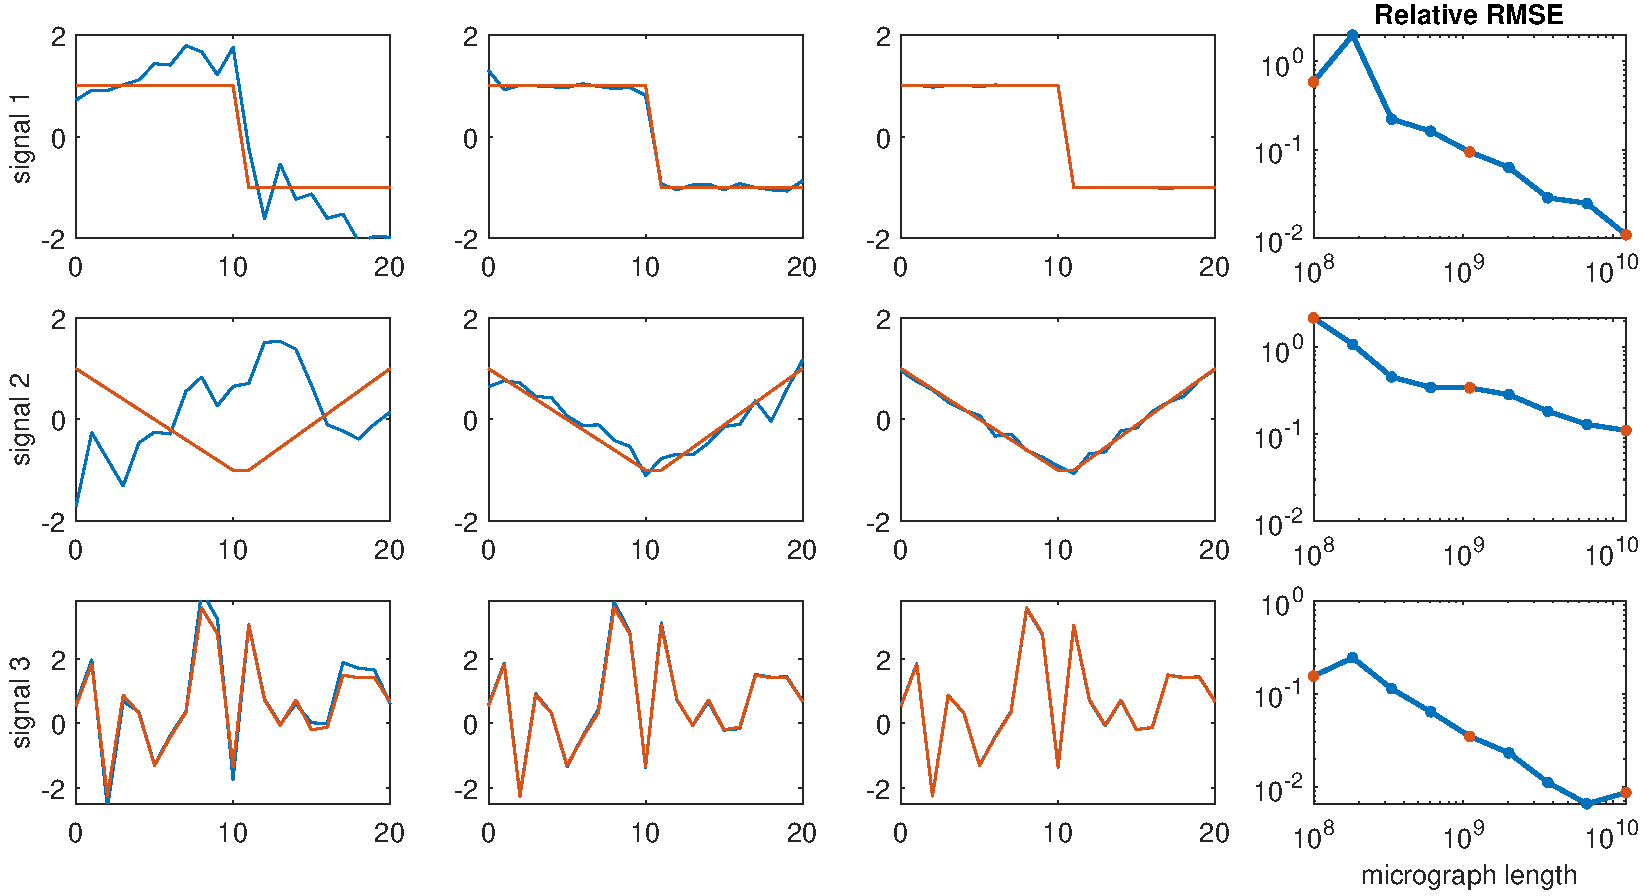
\includegraphics[width=1\linewidth]{heterogeneous_progressive_n12300000000_466300}
	\caption{Experiment described in Section~\ref{sec:XP1}. For a fixed noise level $\sigma = 3$ and a fixed set of $K = 3$ signals of length $L = 21$, an observation $y$ of length $N = 12.3 \cdot 10^9$ is generated according to~\eqref{eq:model} in the well-separated model, with fixed density and occurrence probabilities. Each rows corresponds to one of the signals. The last column shows evolution of the relative root mean squared error in estimating each signal, as a longer and longer subset of $y$ is observed. Red dots mark the three snapshots that are illustrated in columns 1--3: red signals are the ground truth and blue signals are the estimators.}
	\label{fig:1Dheterosignals}
\end{figure}

For the experiment depicted in Figure~\ref{fig:1Dheterosignals}, we fix $K = 3$ signals of length $L = 21$: see the three red signals in the first column. Following~\eqref{eq:model}, we generate an observation $y$ of length $12.3 \cdot 10^9$. Each of the three signals appears, respectively (and approximately), $30.0 \cdot 10^6$, $20.0 \cdot 10^6$ and $10.0 \cdot 10^6$ times in $y$ for a total of exactly $60 \cdot 10^6$ occurrences, such that at least $L-1$ zeros separate any two occurrences of any signals according to~\eqref{eq:spacing}. This is done by randomly selecting $60 \cdot 10^6$ placements in $y$, one at a time with an accept/reject rule based on the separation constraint and locations picked so far. For each placement, one of the three signals is picked at random according to the proportions $\pi = (1/2, 1/3, 1/6)$. Then, i.i.d.\ Gaussian noise with mean zero and standard deviation $\sigma = 3$ is added, to form the observed $y$. The resulting signal-to-noise ratio of $y$
% sqrt((m_want*sum(X.^2)')/(sigma^2*n))
is about 1/9.

Visually, the noise dominates the signal to the point that it is challenging to detect occurrences. More precisely, the cross-correlations of $y$ even with the true signals presents peaks at essentially random locations, apparently uninformative of the actual locations of the signal occurrences. Thus, we contend that it would be difficult for any algorithm to locate the signal occurrences, let alone to classify them according to which signal appears where.

%Given the observation $y$, we proceed to compute the autocorrelations. The first-order autocorrelation is straightforward. For second-order autocorrelations, notice from equation~\eqref{eq:data_ac} that $a_y^2[\ell]$ suffers no noise-induced bias for $\ell$ in $1$ to $L-1$. Thus, we omit $\ell = 0$, which has the practical effect that we need not know $\sigma$ to make sense of the computed quantities. Likewise, for third-order autocorrelations, $a_y^3[\ell_1, \ell_2]$ for $0 \leq \ell_1, \ell_2 \leq L-1$ such that $\ell_2 \leq \ell_1$ includes all relevant entries for our purpose (this accounts for symmetries), and we further exclude any such that $\ell_1, \ell_2$ or $\ell_1 - \ell_2$ are zero to avoid the need to estimate $\sigma$---there are $\frac{(L-1)(L-2)}{2}$ remaining entries. We have
%\begin{align*}
%1 + (L-1) + \frac{(L-1)(L-2)}{2} = \frac{1}{2} L (L-1) + 1
%\end{align*}
%coefficients in total. Since we aim to estimate $KL$ parameters (for the $K$ signals of length $L$) plus $K$ parameters (for the densities $\gamma_k$), an absolute upper bound on $K$ (simply to ensure we have at least as many equations as we have unknowns) is
%\begin{align*}
%K(L+1) \leq \frac{1}{2} L (L-1) + 1.
%\end{align*}
%Thus, $(L-1)/2$ (up to a small approximation) is an absolute upper limit on $K$ (compare with~\cite{boumal2017heterogeneous,bandeira2017estimation}).

Our aim is to investigate how accurately we can estimate the signals as a function of the observation length. To this end, we consider a growing part of the observation $y$. For each length, we compute autocorrelations on that part, then we go on to estimate the signals from these ``mixed'' quantities. In practice, the autocorrelations are computed on disjoint segments of $y$ of length $100\cdot10^6$ and added up, without correction for the junction points. Segments are handled sequentially on a GPU, as GPUs are particularly well suited to execute simple instructions across large vectors of data. If multiple GPUs are available, segments can  be handled in parallel.


Having computed the autocorrelations of interest, we estimate signals $x_1, \ldots, x_K$ and coefficients $\gamma_1, \ldots, \gamma_K$ which agree with the data. We choose to do so by running an optimization algorithm on the following nonlinear least-squares problem:
\begin{multline}
	\min_{\substack{\hat x_1, \ldots, \hat x_K \in \R^{W} \\ \hat \gamma_1, \ldots, \hat \gamma_K > 0}} w_1 \left( a_y^1 - \sum_{k=1}^K \hat \gamma_k a_{\hat x_k}^1 \right)^2 + w_2 \sum_{\ell = 1}^{L-1} \left( a_y^2[\ell] - \sum_{k=1}^K \hat \gamma_k a_{\hat x_k}^2[\ell] \right)^2 + \\ w_3 \sum_{\substack{2\leq\ell_1\leq L-1 \\ 1 \leq \ell_2 \leq \ell_1-1}} \left( a_y^3[\ell_1, \ell_2] - \sum_{k=1}^K \hat \gamma_k a_{\hat x_k}^3[\ell_1,\ell_2] \right)^2,
	\label{eq:optim1D}
\end{multline}
where $W \geq L$ is the length of the sought signals and the weights are set to $w_1 = 1/2, w_2 = 1/2n_2, w_3 = 1/2n_3$, where $n_2, n_3$ are the number of coefficients used for each autocorrelation order: $n_2 = L-1$, $n_3 = \frac{(L-1)(L-2)}{2}$ (weights could also be set in accordance with variance estimates as in~\cite{boumal2017heterogeneous}).

Setting $W = L$ (as is a priori desired) is problematic because the above optimization problems appears to have numerous poor local optimizers. Thus, we first run the optimization with $W = 2L-1$. This problem appears to have few poor local optima, perhaps because the additional degrees of freedom allow for more escape directions. Since we hope the signals estimated this way correspond to the true signals zero-padded on either side to length $W$, we extract from each one a subsignal of length $L$ that has largest $\ell_2$-norm. This estimator is then used as initial iterate for~\eqref{eq:optim1D}, this time with $W = L$. We find that this procedure is reliable for a wide range of experimental parameters. To solve~\eqref{eq:optim1D}, we run the trust-region method implemented in Manopt~\cite{manopt}, which allows to treat the positivity constraints on coefficients $\hat \gamma_k$. Notice that the cost function is a polynomial in the variables, so that it is straightforward to compute it and its derivatives.

In Figure~\ref{fig:1Dheterosignals}, we find that the signals can be recovered with good accuracy despite the noise levels which seemingly preempts location and classification. We also note that the amount of data required to produce these good estimations is large. Furthermore, as illustrated here and as we have observed in numerous experiments, signals with more variations (such as the third signal in this experiment which was generated once from a Gaussian distribution) are easier to estimate accurately than more regular signals (in this case, despite the fact that the third signal occurs less frequently than the others).
This phenomenon has been also observed in multi-reference alignment~\cite[Section 3.2]{perry2017sample}.

\subsection{Experiment 2}

\begin{figure}[t]
	\centering
	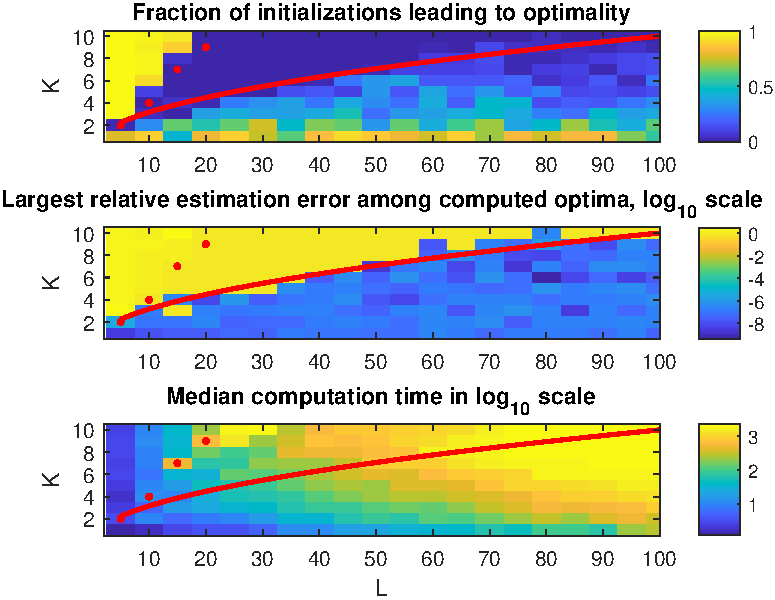
\includegraphics[width=.7\linewidth]{KLXP/XP1}
	\caption{In the $N \to \infty$ regime (access to exact autocorrelations, excluding biased entries) and with known uniform densities, it seems $K$ up to $\sqrt{L}$ (red curve) i.i.d.\ Gaussian signals of length $L$ can be recovered from the known moments. CPU time in seconds. Strictly above red dots, recovery is impossible because the number of unknowns exceeds the number of computed moments. Similar to~\cite[Fig.~4.1]{boumal2017heterogeneous}, this experiment suggests a possible statistical-computational gap.}
	\label{fig:KLXP}
\end{figure}

In this second experiment, presented in Figure~\ref{fig:KLXP}, we investigate how many distinct signals ${x_1, \ldots, x_K}$ can be estimated from mixed autocorrelations~\eqref{eq:mixedautocorr}. In order to do so, we consider a setup where the mixed autocorrelations are known perfectly. This corresponds to the limit of an infinitely long observation $y$ with fixed density $\gamma$ and fixed noise level (that may be arbitrarily high). The specific value of $\sigma$ is immaterial since we only consider autocorrelations that are unaffected by noise bias. Furthermore, we assume uniform occurrence distribution $\pi$ (known to the algorithm), and known density $\gamma$ (which is then irrelevant as it only induces a global scaling of the autocorrelations of $y$).

To produce Figure~\ref{fig:KLXP}, we consider each pair $(K, L)$ in turn, with $K = 1, 2, 3, \ldots, 10$ and $L = 5, 10, 15, \ldots, 100$. For each pair, we generate $K$ random normal signals of length $L$, once. The perfect mixed autocorrelations are computed. They are then provided to the inversion algorithm described in Section~\ref{sec:XP1}, together with the knowledge that signals occur with equal probability, as well as the correct density $\gamma$. The algorithm is initialized 50 times with an independent random initial guess, also following a normal distribution. For each run, we record three metrics:
\begin{enumerate}
	\item Whether the optimization algorithm managed to produce a solution with cost function value below $10^{-16}$: this assesses whether optimization succeeded.
	\item The relative root mean squared error between the estimated signals and the ground truth (up to permutation of the $K$ signals.)
	\item The computation time in seconds (keeping in mind that the 50 runs are done in parallel on the same, shared computer, so that this is more of a qualitative assessment.)
\end{enumerate}
These metrics are summarized and presented in Figure~\ref{fig:KLXP} as three panels.
\begin{enumerate}
	\item Panel 1 shows for each pair $(K, L)$ which fraction of the 50 runs reached optimality (between 0 and 1).
	\item For each pair $(K, L)$, any estimator produced by the optimization algorithm such that the cost function value is close to zero must be considered a valid estimator, since it agrees almost perfectly with the data. For all of those, we compute the error compared to the ground truth. Panel 2 shows the largest such error, on a log scale in base 10. (If optimization never succeeded for that pair, we report a relative error of 1.) A large value means that, among all near global optima of the optimization problem (if any), at least one was a poor estimator. A small value indicates all computed near global optima were good estimators.
	\item Median $\log_{10}$ computation time (where the median is computed after taking the log of the CPU times, in base 10.)
\end{enumerate}

Following~\cite{boumal2017heterogeneous}, overlaid on the panels we trace the red curve $K = \sqrt{L}$ as well as red dots which are computed from the considerations in Section~\ref{sec:heterogeneity} (adapted to the fact that $\pi$ and $\gamma$ are known). We observe that strictly above the red dots the optimization problem appears to be easy to solve (despite non-convexity), yet, as predicted, the corresponding estimators are not informative since there is not enough information in the computed quantities compared to the number of parameters. On the other hand, below the (empirical) red curve, the optimization problem is sometimes solved to optimality (although it may take more than one random initialization to get one successful run), and the corresponding estimators are accurate. In between the red curve and the red dots, the optimization problem appears to be particularly challenging: we essentially never produce a global optimum, hence we also do not have an estimator. This experiment suggests a possible computational-statistical gap in the area between the red curve and the red dots, where it is possible that the signals could be estimated, but perhaps not with a computationally efficient procedure.
Similar results were observed for the multi-reference problem~\cite{boumal2017heterogeneous,weinthesis,bandeira2017estimation}.

\subsection{Experiment 3}

Autocorrelation analysis can be carried out in dimensions greater than one. In the following experiment, we estimate 
a 50-by-50 pixel grayscale picture of Einstein with mean zero from a growing number of observations $y$. Each observation is of size $4096\times 4096$ pixels and contains 700 occurrences on average at random locations, while maintaining the separation condition~\eqref{eq:spacing} in each axis separately.
The observations are contaminated with additive white Gaussian noise with standard deviation $\sigma = 3$, illustrated in Figure~\ref{fig:micro_example}. 
 % corresponding  to SNR = ${\frac{M\|x\|_F^2} {\sigma^2N} \approx1/370}$. 
%As explained in Section~\ref{sec:high_dimensions}, an image is determined uniquely form its second-order autocorrelation.
%Hence, to use this property and keep things simple, we assume the number of signal occurrences and the noise standard deviation are known so that we can estimate the second-order autocorrelation of the image from thos the observation directly.  %Micrographs are generated such that any two occurrences are always separated by at least 49 pixels in each direction in accordance with the separation condition~\eqref{eq:spacing}. 

We compute the average second-order autocorrelation of the observations. This is a particularly simple computation which can be efficiently executed with a fast Fourier transform (FFT), in parallel over the numerous observations. To  keep things simple, we assume the number of signal occurrences (akin to the density $\gamma$) and the standard deviation of the noise, $\sigma$, are known. Given those quantities, the second-order autocorrelation of the image can be easily deduced from~\eqref{eq:ac2_micrograph}. \TODO{As explained in Section~\ref{sec:high_dimensions}---careful if we decide to edit}, an image is determined uniquely form its second-order autocorrelations. Then, to estimate the target image, we use a standard phase retrieval algorithm called relaxed-reflect-reflect (RRR)~\cite{elser2017rrr}, initialized randomly.


\begin{figure}[t]
	\centering
	\begin{subfigure}[h]{0.33\linewidth}
		\centering
		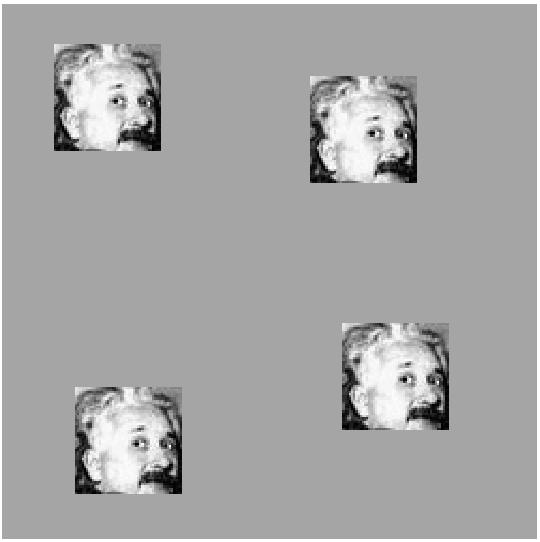
\includegraphics[width=.8\linewidth]{micrograph_Einstein_example_clean}
		\caption{$\sigma = 0$}
	\end{subfigure}%
	\begin{subfigure}[h]{0.33\linewidth}
		\centering
		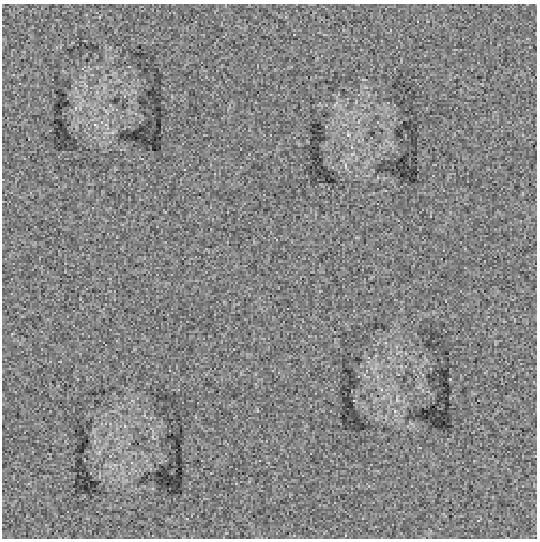
\includegraphics[width=.8\linewidth]{micrograph_Einstein_example_s05}
		\caption{$\sigma = 0.5$}
	\end{subfigure}
	\begin{subfigure}[h]{0.33\linewidth}
		\centering
		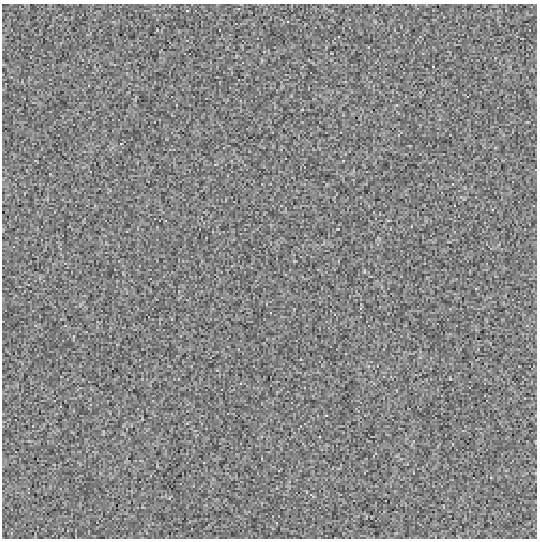
\includegraphics[width=.8\linewidth]{micrograph_Einstein_example_s3}
		\caption{$\sigma = 3$}
	\end{subfigure}
	\caption{\label{fig:micro_example} Example of observations for the 2-D experiment (of size $250\times 250$) with additive white Gaussian noise of variance $\sigma^2$ for increasing values of $\sigma$. Each observation contains the same four occurrences of a $50 \times 50$ image of Einstein. In panel (c), the noise level is such that it is challenging to detect  the planted images.} %In fact, it can be shown that at low SNR, reliable detection of individual image occurrences is impossible, even if the true image is known. } 	
\end{figure}
%By analogy to cryo-EM, this depicts a scenario where particle picking cannot be done.}
%\vspace{-8pt}

Relative error is measured as the ratio of the root mean square error to the norm of the ground truth (square root of the sum of squared pixel intensities). Figure~\ref{fig:Einst_example} shows several estimated images for a growing number of observations. Figure~\ref{fig:error_per_micro} presents the normalized recovery error as a function of the amount of data available.  This is computed after fixing the reflection symmetries (see Section~\ref{sec:high_dimensions}).

As evidenced by these figures, the ground truth image can be estimated increasingly well from increasingly many observations, without the need to locate the signal occurrences.



\begin{figure}[t]
	\centering
	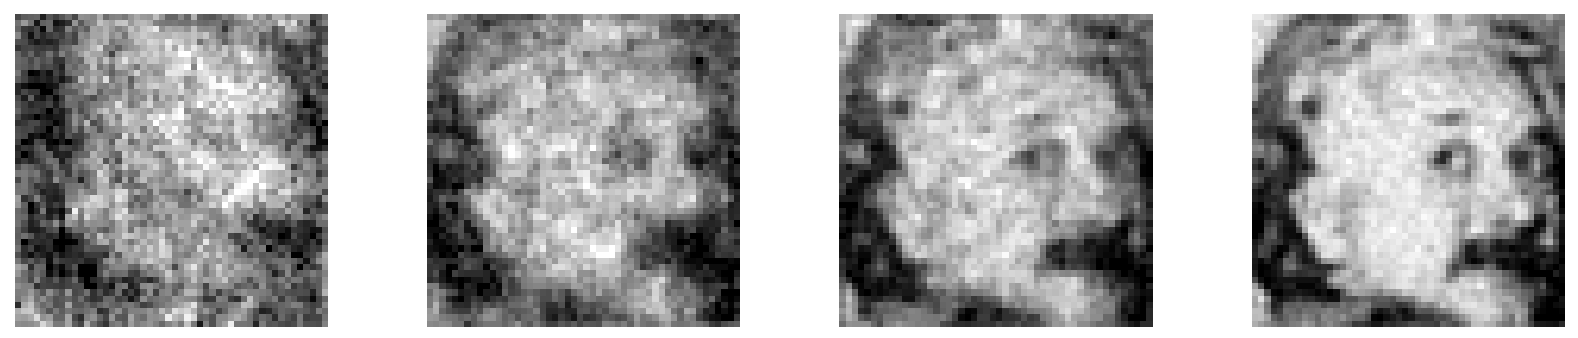
\includegraphics[width=1\linewidth]{Einstien_progress_examples}
	\caption{\label{fig:Einst_example} Recovery of Einstein from observations at noise level $\sigma = 3$ (see Figure~\ref{fig:micro_example}(c)). Averaged autocorrelations of the data allow to estimate the power spectrum of the target image. This does not require locating the signal occurrences. The RRR algorithm produces the estimates,  obtained from $2\times 10^2,2\times 10^3,2\times 10^4$ and $2\times 10^5$ observations (growing across panels from left to right).}	
	%	\vspace{-8pt} 
\end{figure}


\begin{figure}[h]
	\centering
	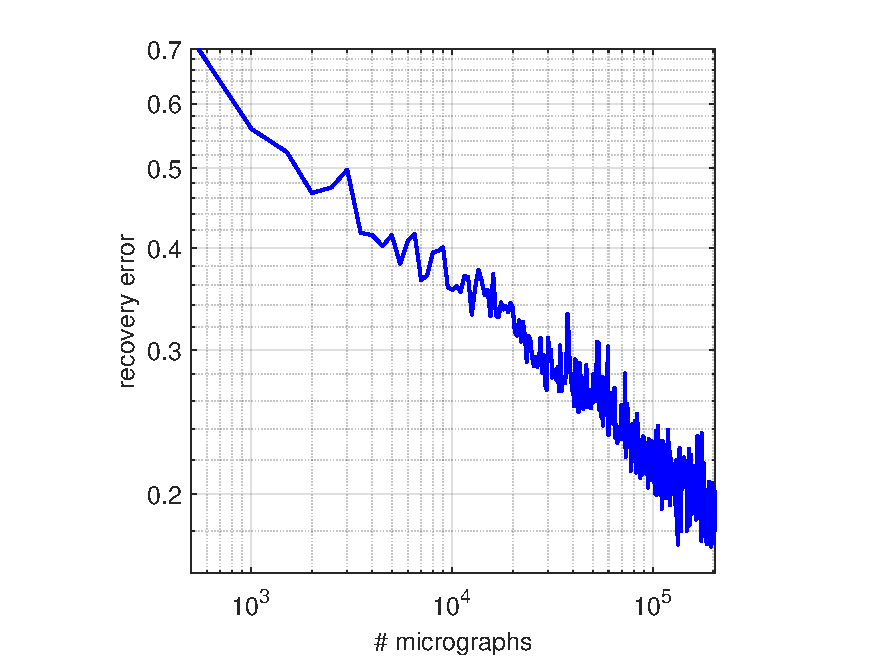
\includegraphics[width=.8\linewidth]{Einstein_recovery_error}
	\caption{\label{fig:error_per_micro}Relative error curve for Experiment 3 in Figure~\ref{fig:Einst_example}. Each observation contains about 700 image occurrences at unknown locations.}
\end{figure}

\section{Proofs}

Proofs for some of the results presented in Section~\ref{sec:AC_analysis} and~\ref{sec:extensions} follow in this section.

\subsection{Autocorrelations in the well-separated model} \label{sec:autocorrelation_computation}

%Let us define
%\begin{equation*}
%\gamma = \frac{|s|L}{N}>0.
%\end{equation*}
%Then the first order autocorrelation of the observation is given by 
%\begin{equation*}
%a_y^1 = \E_y\left\{\frac{1}{N}\sum_{i=0}^{N-1} y[i]\right\} =
%\frac{|s|}{N}\E_x\left\{\sum_{i=0}^{L-1}x[i]\right\} +    
%\E_{\varepsilon}\left\{\frac{1}{N}\sum_{i=0}^{N-1}\varepsilon[i]\right\}
%=\gamma a_x^1,
%\end{equation*}
%where $\E_z$ means expectation with respect to the distribution of $z$.
%%the noise term converges to zero almost surely (a.s.)\ by the strong law of large numbers.
%
%We proceed with the second-order autocorrelation for  $\ell\in\{0,\ldots,L-1\}$. We can compute:
%%
%\begin{align*}
%%
%a_y^2[\ell] & = \E_y\left\{\frac{1}{N}\sum_{i=0}^{N-1-\ell}y[i]y[i+\ell]\right\}
%\nonumber \\
%& = \frac{|s|}{N}\E_x\left\{\sum_{i=0}^{L-\ell-1}x[i]x[i+\ell]\right\}  + \E_{\varepsilon}\left\{\frac{1}{N}\sum_{i=0}^{N-1-\ell}\varepsilon[i]\varepsilon[i+\ell] \right\},
%%
%\end{align*}
%where all cross terms vanish in expectation owing to independence of $x$ of $\varepsilon$, and $\E{\varepsilon}=0$.  
%Hence, 
%\begin{align} \label{eq:2nd_moment_signal_term}
%%
%a_y^2[\ell] & = \gamma a_x^2[\ell] + \frac{N-1-\ell}{N}\sigma^2\delta[\ell],
%\end{align}
%where $\delta[0]=1$ and zero otherwise. 
%
%We now analyze the third-order autocorrelation. 
%Let $x_{(j)}$ denote the $j$th
%realization of $x$, with starting position $s_{(j)}$, for $j=1,\ldots,|s|$.
%Let us fix $0\leq \ell_2\leq\ell_1\leq L-1$. We have:
%\begin{align*}
%%
%a_y^3[\ell_1,\ell_2] 
%=& \E_y\left\{\frac{1}{N}\sum_{i=0}^{N-1-\ell_1} y[i]y[i+\ell_1]y[i+\ell_2]\right\}
%\\
%%
%\stackrel{(1)}=& \E_{x_{(1)},\ldots,x_{(|s|)}}\left\{ \frac{|s|L}{N}\frac{1}{|s|}\sum_{j=1}^{|s|} 
%	\frac{1}{L}\sum_{i=0}^{L-1-\ell_1}x_{(j)}[i]x_{(j)}[i+\ell_1]x_{(j)}[i+\ell_2]  \right\} \\
%\stackrel{(2)}+& \E_\varepsilon\left\{\frac{1}{N}\sum_{i=0}^{N-1-\ell_1} \ep[i]\ep[i+\ell_1]\ep[i+\ell_2]\right\}
%\ \\
%\stackrel{(3)}+& \E_{x_{(1)},\ldots,x_{(|s|)},\varepsilon}\left\{\frac{1}{N}\sum_{j=1}^{|s|} 
%	\sum_{i=0}^{L-1} x_{(j)}[i]\ep[s_{(j)} + i+\ell_1]\ep[s_{(j)}+ i+\ell_2]\right\} \\
%\stackrel{(4)}+& \E_{x_{(1)},\ldots,x_{(|s|)},\varepsilon}\left\{\frac{1}{N}\sum_{j=1}^{|s|} 
%	\sum_{i=0}^{L-1} \ep[s_{(j)}+i-\ell_1]x_{(j)}[i]\ep[s_{(j)}+ i+\ell_2-\ell_1]\right\}
%\\
%\stackrel{(5)}+& \E_{x_{(1)},\ldots,x_{(|s|)},\varepsilon}\left\{\frac{1}{N}\sum_{j=1}^{|s|} 
%	\sum_{i=0}^{L-1} \ep[s_{(j)}+i-\ell_2]\ep[s_{(j)}+i+\ell_1-\ell_2]x_{(j)}[i]\right\}
%\\ \stackrel{(6)}+ & \E_{x_{(1)},\ldots,x_{(|s|)},\varepsilon}\left\{\frac{1}{N}\sum_{j=1}^{|s|} 
%	\sum_{i=0}^{L-\ell_1+\ell_2-1} \ep[s_{(j)}+i-\ell_2]x_{(j)}[i+\ell_1-\ell_2]x_{(j)}[i]\right\}
%\\
%\stackrel{(7)}+ & \E_{x_{(1)},\ldots,x_{(|s|)},\varepsilon}\left\{\frac{1}{N}\sum_{j=1}^{|s|} 
%	\sum_{i=0}^{L-\ell_2-1} x_{(j)}[i]\ep[s_{(j)} + i+\ell_1]x_{(j)}[i+\ell_2]\right\}
%\\ \stackrel{(8)}+ & \E_{x_{(1)},\ldots,x_{(|s|)},\varepsilon}\left\{\frac{1}{N}\sum_{j=1}^{|s|} 
%	\sum_{i=0}^{L-\ell_1-1} x_{(j)}[i]x_{(j)}[i+\ell_1]\ep[s_{(j)}+ i+\ell_2]\right\}.
%%
%\end{align*}
%Terms (6), (7) and (8) are linear in $\ep$ and  thus zero.
%Term (1) is equal  to $\gamma a_x^3[\ell_1,\ell_2]$  for the same reasons as~\eqref{eq:2nd_moment_signal_term}. 
%Term (2) is always zero by properties of Gaussian variables. 
%To deal with terms (3)--(5), we must distinguish between different values of $\ell_1$ and $\ell_2$.
%
%Term (3) is always zero, unless $\ell_1=\ell_2$, so that it is equal to 
%$\gamma\sigma^2 a_x^1 \delta[\ell_1-\ell_2]$.
%The same goes for Terms (4) and (5), which are equal, respectively, to
%$\gamma\sigma^2 a_x^1 \delta[\ell_2]$ 
%and $\gamma\sigma^2 a_x^1 \delta[\ell_1]$.


Let $x_{(1)}, \ldots, x_{(|s|)}$ denote the (independent) realizations of the random signal $x$ in the observation $y$, starting at (deterministic) positions $s_{(1)}, \ldots, s_{(|s|)}$. Let $I_{ij}$ be the indicator variable for whether position $i$ is in the support of occurrence $j$, that is, it is one if $i$ is in $\{s_{(j)}, \ldots, s_{(j)}+L-1\}$, and zero otherwise. Then,
\begin{align}
y[i] & = \sum_{j = 1}^{|s|} I_{ij} x_{(j)}[i-s_{(j)}] + \varepsilon[i].
\label{eq:explicityiindicators}
\end{align}
This gives a simple expression for the first autocorrelation of $y$. Indeed,
\begin{align}
a_y^1 & = \E_y\left\{ \frac{1}{N} \sum_{i = 0}^{N-1} y[i] \right\} \\
& = \frac{1}{N} \E_{x_{(1)}, \ldots, x_{(|s|)}, \varepsilon}\left\{ \sum_{i = 0}^{N-1} \sum_{j = 1}^{|s|} I_{ij} x_{(j)}[i-s_{(j)}] + \varepsilon[i] \right\}.
\end{align}
Now switch the sums over $i$ and $j$, and observe that $I_{ij}$ is zero unless $i = s_{(j)} + t$ for $t$ in the range $0, \ldots, L-1$. Hence,
\begin{align}
a_y^1 & = \frac{1}{N} \sum_{j = 1}^{|s|} \E_{x_{(j)}}\left\{ \sum_{t = 0}^{L-1} x_{(j)}[t]\right\} + \frac{1}{N} \E_\varepsilon\left\{ \sum_{i=0}^{N-1} \varepsilon[i]\right\}.
\end{align}
Since the noise has zero mean and $x_{(1)}, \ldots, x_{(|s|)}$ are independent and all distributed as $x$, we further find:
\begin{align}
a_y^1 & = \frac{|s|L}{N} a_x^1 = \gamma a_x^1.
\end{align}

To address the second-order moments, we resort to the separation conditions. First, consider this expression:
\begin{align*}
N \cdot a_y^2[\ell] & = \E_y\left\{ \sum_{i = 0}^{N-\ell-1} y[i] y[i+\ell] \right\} \\
& = \sum_{i = 0}^{N-\ell-1} \E_{x_{(1)}, \ldots, x_{(|s|)}, \varepsilon}\Bigg\{ \left( \sum_{j = 1}^{|s|} I_{ij} x_{(j)}[i-s_{(j)}] + \varepsilon[i] \right) \cdot \\
& \qquad \qquad \qquad \qquad \qquad  \left( \sum_{j' = 1}^{|s|} I_{i+\ell,j'} x_{(j')}[i+\ell-s_{(j')}] + \varepsilon[i+\ell] \right)  \Bigg\} \\
& = \sum_{i = 0}^{N-\ell-1} \E_{x_{(1)}, \ldots, x_{(|s|), \varepsilon}}\Bigg\{ \sum_{j = 1}^{|s|} \sum_{j' = 1}^{|s|} I_{ij}  I_{i+\ell,j'} x_{(j)}[i-s_{(j)}]  x_{(j')}[i+\ell-s_{(j')}] \\
& \qquad \qquad \qquad \qquad \qquad \qquad + \sum_{j = 1}^{|s|} I_{ij} x_{(j)}[i-s_{(j)}] \varepsilon[i+\ell] \\
& \qquad \qquad \qquad \qquad \qquad \qquad + \sum_{j' = 1}^{|s|} I_{i+\ell,j'} x_{(j')}[i+\ell-s_{(j')}] \varepsilon[i] \\
& \qquad \qquad \qquad \qquad \qquad \qquad + \varepsilon[i] \varepsilon[i + \ell] \Bigg\}.
\end{align*}
The cross-terms vanish in expectation since $\varepsilon$ is zero mean and independent from the signal occurrences. The last term vanishes in expectation unless $\ell = 0$ since distinct entries of $\varepsilon$ are independent. For $\ell = 0$, $\E\{\varepsilon[i]^2\} = \sigma^2$. Finally, using the separation property, observe that if $I_{ij}  I_{i+\ell,j'}$ is nonzero, then it is equal to one, $j = j'$ and $i = s_{(j)} + t$ for some $t$ in $0, \ldots, L-\ell-1$. Then, switch the order of summations to get
\begin{align}
N \cdot a_y^2[\ell] & = \sum_{j=1}^{|s|} \E_{x_{(j)}}\left\{ \sum_{t = 0}^{L-\ell-1} x_{(j)}[t] x_{(j)}[t+\ell] \right\} + (N-\ell)\sigma^2 \delta[\ell],
\end{align}
where $\delta[0] = 1$ and $\delta[\ell \neq 0] = 0$. Since each $x_{(j)}$ is distributed as $x$, they all have the same autocorrelations as $x$ and we finally get
\begin{align}
a_y^2[\ell] & = \gamma a_x^2[\ell] + \frac{N-\ell}{N}\sigma^2 \delta[\ell] = \gamma a_x^2[\ell] + \sigma^2 \delta[\ell].
\end{align}

We now turn to the third-order autocorrelations. These involve the sum
\begin{align}
\sum_{i=0}^{N-\max(\ell_1, \ell_2)-1} y[i] y[i+\ell_1] y[i+\ell_2].
\end{align}
Using~\eqref{eq:explicityiindicators}, we find that this quantity can be expressed as a sum of eight terms:
% \sum_{j = 1}^{|s|} I_{ij} x_{(j)}[i-s_{(j)}] + \varepsilon[i]
\begin{enumerate}
	\item $\sum_i \sum_{j,j',j'' = 1}^{|s|} I_{ij} I_{i+\ell_1, j'} I_{i+\ell_2,j''} x_{(j)}[i-s_{(j)}] x_{(j')}[i+\ell_1-s_{(j')}] x_{(j'')}[i+\ell_2-s_{(j'')}]$
	\item $\sum_i \sum_{j,j' = 1}^{|s|} I_{ij} I_{i+\ell_1, j'} x_{(j)}[i-s_{(j)}] x_{(j')}[i+\ell_1-s_{(j')}] \varepsilon[i+\ell_2]$
	\item $\sum_i \sum_{j,j'' = 1}^{|s|} I_{ij} I_{i+\ell_2,j''} x_{(j)}[i-s_{(j)}] \varepsilon[i+\ell_1] x_{(j'')}[i+\ell_2-s_{(j'')}]$
	\item $\sum_i \sum_{j',j'' = 1}^{|s|} I_{i+\ell_1, j'} I_{i+\ell_2,j''} \varepsilon[i] x_{(j')}[i+\ell_1-s_{(j')}] x_{(j'')}[i+\ell_2-s_{(j'')}]$
	\item $\sum_i \sum_{j = 1}^{|s|} I_{ij} x_{(j)}[i-s_{(j)}] \varepsilon[i+\ell_1] \varepsilon[i+\ell_2]$
	\item $\sum_i \sum_{j' = 1}^{|s|} I_{i+\ell_1, j'} \varepsilon[i] x_{(j')}[i+\ell_1-s_{(j')}] \varepsilon[i+\ell_2]$
	\item $\sum_i \sum_{j'' = 1}^{|s|} I_{i+\ell_2,j''} \varepsilon[i] \varepsilon[i+\ell_1] x_{(j'')}[i+\ell_2-s_{(j'')}]$
	\item $\sum_i \varepsilon[i] \varepsilon[i+\ell_1] \varepsilon[i+\ell_2]$
\end{enumerate}
Terms 2--4 and 8 vanish in expectation since odd moments of centered Gaussian variables are zero. For the first term, we use the fact that the separation condition implies
\begin{multline}
I_{ij} I_{i+\ell_1, j'} I_{i+\ell_2,j''} = 1 \iff \\ j=j'=j'' \textrm{ and } i = s_{(j)} + t \textrm{ with } t \in \{ 0, \ldots L-\max(\ell_1, \ell_2)-1 \}.
\end{multline}
(Otherwise, the product of indicators is zero.) This allows to reduce the summations over $j,j',j''$ to a single sum over $j$. Then, witching the order of summation with $i$, we get that the first term is equal to
\begin{align}
\sum_{j=1}^{|s|} \sum_{t=0}^{L-\max(\ell_1, \ell_2)-1} x_{(j)}[t] x_{(j)}[t+\ell_1] x_{(j)}[t+\ell_2].
\end{align}
In expectation over the realizations $x_{(j)}$, using again that they are i.i.d.\ with the same distribution as $x$, this first term yields $|s|L a_x^3[\ell_1, \ell_2]$. Now consider the fifth term. Taking expectation against $\varepsilon$ yields
\begin{align}
\sum_{i=0}^{N-\max(\ell_1, \ell_2)-1} \sum_{j = 1}^{|s|} I_{ij} x_{(j)}[i-s_{(j)}] \sigma^2 \delta[\ell_1 - \ell_2].
\end{align}
Switch the order of summation over $i$ and $j$ again to get
\begin{align}
\sigma^2 \delta[\ell_1 - \ell_2] \sum_{j = 1}^{|s|} \sum_{t=0}^{L-1} x_{(j)}[t].
\end{align}
Now taking expectation against the signal occurrences yields $|s|L \sigma^2 a_x^1 \delta[\ell_1 - \ell_2]$. A similar reasoning for terms 6 and 7 yields this final formula for the third-order autocorrelations of $y$:
\begin{align}
a_y^3[\ell_1, \ell_2] & = \gamma a_x^3[\ell_1, \ell_2] + \gamma \sigma^2 a_x^1 \left( \delta[\ell_1] + \delta[\ell_2] + \delta[\ell_1 - \ell_2] \right).
\end{align}


\subsection{Autocorrelations in the Poisson model} \label{sec:proof_prop_poisson}

\TODO{Needs a complete rewrite to match the paper, in particular the modified notation and the fact we only work with autocorrelations now (not models).}

\subsubsection{First moment}

To compute the first moment of $y$, we will first condition on $M = (M_1,\dots,M_{N-L+1})$, and then average over $M$. We have:
%
\begin{align}
%
\E[y[i] | M] = \sum_{j=0}^{L-1} \sum_{k=1}^{M_{i-j}} \E X_k^{i-j}[j]
= \sum_{j=0}^{L-1} \sum_{k=1}^{M_{i-j}} m_y^1[j]
= \sum_{j=0}^{L-1} M_{i-j} m_y^1[j].
%
\end{align}
%
Now taking expectations over $M$ we see:
%
\begin{align}
%
\E Y[i] = \gamma \sum_{j=0}^{L-1}  m_y^1[j] = \gamma La_x^1.
%
\end{align}


%


\subsubsection{Second moment}

Again, we will condition on $M$ first, and then take the expectation over $M$. Fix $i_1 \ne i_2$, and let $\Delta = i_2 - i_1$. Then:
%
\begin{align}
%
Y_{i_1} Y_{i_2} 
&= \sum_{j_1=0}^{L-1} \sum_{j_2=0}^{L-1} 
\sum_{k_1=1}^{M_{i_1-j_1}}\sum_{k_2=1}^{M_{i_2-j_2}}
X_{k_1}^{i_1-j_1}[j_1] X_{k_2}^{i_2 - j_2}[j_2].
%
\end{align}

We break up the double sum over $j_1$ and $j_2$ into two terms: one where $j_2 \ne j_1 + \Delta$, and one where $j_2 = j_1 + \Delta$ or equivalently $i_1-j_1 = i_2-j_2$. In the first case, all the terms are independent, and so the expectation factors. In the second case, when $k_1 \ne k_2$ we have independence, but otherwise not. This gives (all expectations are conditional on $M$):
%
\begin{align} \label{moment2-condm}
%
\E Y_{i_1} Y_{i_2}
=& \sum_{j_1=0}^{L-1} \sum_{j_2=0}^{L-1} 
\sum_{k_1=1}^{M_{i_1-j_1}}\sum_{k_2=1}^{M_{i_2-j_2}}
\E X_{k_1}^{i_1-j_1}[j_1] X_{k_2}^{i_2 - j_2}[j_2]
\nonumber \\
=& \sum_{j_1 - j_2 \ne \Delta} \sum_{k_1} 
\sum_{k_2} \E X_{k_1}^{i_1-j_1}[j_1] X_{k_2}^{i_2 - j_2}[j_2]
\nonumber \\
& + \sum_{j_1 = 0}^{L-1} \sum_{k_1 \ne k_2} 
\E X_{k_1}^{i_1-j_1}[j_1] X_{k_2}^{i_1 - j_1}[j_1+\Delta]
\nonumber \\
& + \sum_{j_1 = 0}^{L-1} \sum_{k_1=1}^{M_{i_1-j_1}} 
\E X_{k_1}^{i_1-j_1}[j_1] X_{k_1}^{i_1-j_1}[j_1 + \Delta] 
\nonumber \\
=& \sum_{j_1 - j_2 \ne \Delta} M_{i_1-j_1} M_{i_2 - j_2} \M_1[j_1] \M_1[j_2]
\nonumber \\
& + \sum_{j_1 = 0}^{L-1} M_{i_1-j_1}(M_{i_1-j_1} - 1) \M_1[j_1] \M_1[j_1 + \Delta]
\nonumber \\
& + \sum_{j_1 = 0}^{L-1} M_{i_1-j_1} \M_2[j_1,j_1 + \Delta] .
%
\end{align}
%
Now take expectations over the Poisson random variables, using this fact:
%
\begin{lem} \label{lem-choose}
	If $M \sim \Poisson(\gamma)$, then 
	\begin{align}
	%
	\E {M\choose k} = \frac{\gamma^k}{k!}.
	%
	\end{align}
\end{lem}


We get (now the expectation is over $M$ and $X$):
%
\begin{align}
%
\E Y_{i_1} Y_{i_2} 
=& \sum_{j_1 - j_2 \ne \Delta} \E M_{i_1-j_1} M_{i_2 - j_2} \M_1[j_1] \M_1[j_2]
\nonumber \\
& + \sum_{j_1 = 0}^{L-1} \E M_{i_1-j_1}(M_{i_1-j_1} - 1) \M_1[j_1] \M_1[j_1 + \Delta]
\nonumber \\
& + \sum_{j_1 = 0}^{L-1} \E M_{i_1-j_1} \M_2[j_1,j_1 + \Delta]
\nonumber \\
=& \sum_{j_1 - j_2 \ne \Delta} \gamma^2 \M_1[j_1] \M_1[j_2]
+ \sum_{j_1 = 0}^{L-1} \gamma^2 \M_1[j_1] \M_1[j_1 + \Delta]
\nonumber \\
& + \sum_{j_1 = 0}^{L-1} \gamma \M_2[j_1,j_1 + \Delta]
\nonumber \\
=&  \bigg(\gamma \sum_{j = 0}^{L-1} \M_1[j] \bigg)^2
+ \gamma \sum_{j = 0}^{L-1} \M_2[j,j + \Delta]
\nonumber \\
=&  (\gamma \L_1)^2 + \gamma \L_2(\Delta).
%
\end{align}

But the first term in the sum is just the square of the first moment of $Y$; so from the first two moments we can recover $\gamma \L_2(\Delta)$, which is just the expected power spectrum of the random vector $X$, i.e.\ the usual second moment we have been working with.


%


\subsubsection{Third moment}

For three distinct $i_1$, $i_2$ and $i_3$, we let $\Delta_1 = i_2 - i_1$ and $\Delta_2 = i_3 - i_1$. We have:
%
\begin{align}
%
&Y_{i_1} Y_{i_2} Y_{i_3}
\nonumber \\
&= \sum_{j_1=0}^{L-1} \sum_{j_2=0}^{L-1} \sum_{j_3=0}^{L-1} 
\sum_{k_1=1}^{M_{i_1-j_1}}\sum_{k_2=1}^{M_{i_2-j_2}} \sum_{k_3=1}^{M_{i_3-j_3}}
X_{k_1}^{i_1-j_1}[j_1] X_{k_2}^{i_2 - j_2}[j_2] X_{k_3}^{i_3 - j_3}[j_3].
\end{align}
%
We will break up the outer three sums into disjoint sums with the following ranges of indices:
%
\begin{enumerate}
	
	\item \label{case1}
	$j_2 = j_1 + \Delta_1$ and $j_3 = j_2 + \Delta_2 - \Delta_1$.
	
	\item \label{case2}
	$j_2 = j_1 + \Delta_1$ and $j_3 \ne j_2 + \Delta_2 - \Delta_1$.
	
	\item \label{case3}
	$j_2 \ne j_1 + \Delta_1$ and $j_3 = j_1 + \Delta_2$.
	
	\item \label{case4}
	$j_2 \ne j_1 + \Delta_1$ and $j_3 \ne j_1 + \Delta_2$ and $j_3 = j_2 + \Delta_2 - \Delta_1$.
	
	\item \label{case5}
	$j_2 \ne j_1 + \Delta_1$ and $j_3 \ne j_1 + \Delta_2$ and $j_3 \ne j_2 + \Delta_2 - \Delta_1$.
	
\end{enumerate}


For Case \ref{case1}, we have $\ell \equiv i_1 - j_1 = i_2 - j_2 = i_3 - j_3$. We further break up the sum:
%
\begin{align}
%
&\sum_{j=0}^{L-1} \sum_{k_1=1}^{M_\ell} \sum_{k_2=1}^{M_\ell} \sum_{k_3=1}^{M_\ell} 
X_{k_1}^{\ell}[j] X_{k_2}^{\ell}[j + \Delta_1] X_{k_3}^{\ell}[j + \Delta_2]
\nonumber \\
=& \underbrace{ \sum_{j=0}^{L-1} \sum_{k_i \text{distinct}} 
	X_{k_1}^{\ell}[j] X_{k_2}^{\ell}[j + \Delta_1] X_{k_3}^{\ell}[j + \Delta_2]
}_{\text{(a)}}
\nonumber \\
&+\underbrace{ \sum_{j=0}^{L-1} \sum_{k_1=k_2\ne k_3} 
	X_{k_1}^{\ell}[j] X_{k_2}^{\ell}[j + \Delta_1] X_{k_3}^{\ell}[j + \Delta_2]
}_{\text{(b)}}
\nonumber \\
&+\underbrace{ \sum_{j=0}^{L-1} \sum_{k_1=k_3\ne k_2} 
	X_{k_1}^{\ell}[j] X_{k_2}^{\ell}[j + \Delta_1] X_{k_3}^{\ell}[j + \Delta_2]
}_{\text{(c)}}
\nonumber \\
&+\underbrace{ \sum_{j=0}^{L-1} \sum_{k_2=k_3\ne k_1} 
	X_{k_1}^{\ell}[j] X_{k_2}^{\ell}[j + \Delta_1] X_{k_3}^{\ell}[j + \Delta_2]
}_{\text{(d)}}
\nonumber \\
&+\underbrace{ \sum_{j=0}^{L-1} \sum_{k_1=k_2=k_3} 
	X_{k_1}^{\ell}[j] X_{k_2}^{\ell}[j + \Delta_1] X_{k_3}^{\ell}[j + \Delta_2]
}_{\text{(e)}}.
%
\end{align}

For term (a), the expectation conditional on $M$ is:
%
\begin{align}
%
\sum_{j=0}^{L-1} M_\ell(M_\ell-1)(M_\ell-2)\M[j] \M[j+\Delta_1] \M[j+\Delta_2].
%
\end{align}
%
Using Lemma \ref{lem-choose}, the unconditional expectation of (a) is then:
%
\begin{align} \label{aaaa}
%
\gamma^3 \sum_{j=0}^{L-1} \M_1[j] \M_1[j+\Delta_1] \M_1[j+\Delta_2].
%
\end{align}


For term (b), the expectation conditional on $M$ is:
%
\begin{align}
%
\sum_{j=0}^{L-1} M_\ell (M_\ell - 1) \M_2[j,j+\Delta_1] \M_1[j + \Delta_2]
%
\end{align}
%
and then again using Lemma \ref{lem-choose} we get the expected value:
%
\begin{align} \label{bbbb}
%
\gamma^2 \sum_{j=0}^{L-1} \M_2[j,j+\Delta_1] \M_1[j+\Delta_2].
%
\end{align}

Similarly, the expected values of terms (c) and (d) are:
%
\begin{align} \label{cccc}
%
\gamma^2 \sum_{j=0}^{L-1} \M_2[j,j+\Delta_2] \M_1[j+\Delta_1].
%
\end{align}
%
and
%
\begin{align} \label{dddd}
%
\gamma^2 \sum_{j=0}^{L-1} \M_2[j+\Delta_1,j+\Delta_2] \M_1[j].
%
\end{align}

Finally, the expected value of term (e) is easily shown to be:
%
\begin{align} \label{eeee}
%
\gamma \sum_{j=0}^{L-1} \M_3[j,j+\Delta_1,j+\Delta_2].
%
\end{align}
%
This concludes the computation for Case \ref{case1}.

Moving onto Case \ref{case2}, we have $\ell_1 \equiv i_1 - j_1 = i_2 - j_2$, and also define $\ell_2 \equiv i_3 - j_3$. By definition, $\ell_1 \ne \ell_2$. The sum is:
%
\begin{align}
%
& \sum_{j_1=0}^{L-1} \sum_{j_3 \ne j_1 + \Delta_2}
\sum_{1 \le k_1,k_2 \le M_{\ell_1}} \sum_{k_3=1}^{M_{\ell_2}}
X_{k_1}^{\ell_1}[j_1] X_{k_2}^{\ell_1}[j_1 + \Delta_1] X_{k_3}^{\ell_2}[j_3]   
\nonumber \\
=& \sum_{j_1=0}^{L-1} \sum_{j_3 \ne j_1 + \Delta_2} \sum_{k_3=1}^{M_{\ell_2}}
\Bigg\{
\sum_{1 \le k_1 \ne k_2 \le M_{\ell_1}} 
X_{k_1}^{\ell_1}[j_1] X_{k_2}^{\ell_1}[j_1 + \Delta_1] X_{k_3}^{\ell_2}[j_3]
\nonumber \\
&       + \sum_{k_1=1}^{M_{\ell_1}} X_{k_1}^{\ell_1}[j_1] X_{k_1}^{\ell_1}[j_1 + \Delta_1] 
X_{k_3}^{\ell_2}[j_3]  \Bigg\}.
%
\end{align}
%
Taking expectations conditional on $M$, we then get:
%
\begin{align}
%
& \sum_{j_1=0}^{L-1} \sum_{j_3 \ne j_1 + \Delta_2} 
\Bigg(M_{\ell_1} (M_{\ell_1}-1) M_{\ell_2} \M_1[j_1] \M_1[j_1 + \Delta_1] \M_1[j_3]
\nonumber \\
&       + M_{\ell_1} M_{\ell_2} \M_2[j_1,j_1+\Delta_1] \M_1[j_3] \Bigg).
%
\end{align}

Taking expectations over $M$ and using Lemma \ref{lem-choose} then gives:
%
\begin{align}
%
& \gamma^3 \sum_{j_1=0}^{L-1} \sum_{j_3 \ne j_1 + \Delta_2} 
\M_1[j_1] \M_1[j_1 + \Delta_1] \M_1[j_3]
\label{ffff} \\
& + \gamma^2 \sum_{j_1=0}^{L-1} \sum_{j_3 \ne j_1 + \Delta_2}  
\M_2[j_1,j_1+\Delta_1] \M_1[j_3].
\label{gggg}
%
\end{align}


Similarly, Cases \ref{case3} and \ref{case4} give the expressions:
%
\begin{align}
%
& \gamma^3 \sum_{j_1=0}^{L-1} \sum_{j_2 \ne j_1 + \Delta_1} 
\M_1[j_1] \M_1[j_1 + \Delta_2] \M_1[j_2]
\label{hhhh} \\
& + \gamma^2 \sum_{j_1=0}^{L-1} \sum_{j_2 \ne j_1 + \Delta_1}  
\M_2[j_1,j_1+\Delta_2] \M_1[j_2]
\label{iiii}
%
\end{align}
%
and
%
\begin{align}
%
& \gamma^3 \sum_{j_2=0}^{L-1} \sum_{j_1 \ne j_2} 
\M_1[j_1] \M_1[j_2 + \Delta_1] \M_1[j_2 + \Delta_2]
\label{jjjj}\\
& + \gamma^2 \sum_{j_2=0}^{L-1} \sum_{j_1 \ne j_2}  
\M_2[j_2+\Delta_1,j_2+\Delta_2] \M_1[j_1].
\label{kkkk}
%
\end{align}

Finally, in Case \ref{case5} we have $i_1 - j_1$, $i_2 - j_2$, and $i_3 - j_3$ are all pairwise distinct. Consequently, the $X$ variables are always independent, and the expectation conditional on $M$ (letting $\ell_q = i_q - j_q$, $q=1,2,3$),
%
\begin{align}
%
\sum_{j_1,j_2,j_3} M_{\ell_1} M_{\ell_2} M_{\ell_3} \M_1[j_1] \M_1[j_2] \M_1[j_3];
%
\end{align}
%
since the $M_{\ell_q}$'s are pairwise independent, $q=1,2,3$, the expectation over $M$ then yields:
%
\begin{align} \label{llll}
%
\gamma^3 \sum_{j_1,j_2,j_3} \M_1[j_1] \M_1[j_2] \M_1[j_3].
%
\end{align}

Now we add all the terms from Cases \ref{case1} to \ref{case5}. Expressions \eqref{aaaa}, \eqref{ffff}, \eqref{hhhh}, \eqref{jjjj}, and \eqref{llll} sum to the expression:
%
\begin{align}
%
(\gamma \L_1)^3.
%
\end{align}

Note that this is obtained directly from the first moment. Expressions \eqref{bbbb}, \eqref{cccc}, \eqref{dddd}, \eqref{gggg},\eqref{iiii}, and \eqref{kkkk} sum to the expression:
%
\begin{align}
%
\gamma \L_1  \cdot 
( \gamma\L_2(\Delta_1) + \gamma\L_2(\Delta_2) + \gamma\L_2(\Delta_2-\Delta_1)).
%
\end{align}
%
Again, note that this is obtained directly from the first two moments. Finally, expression \eqref{eeee} is simply:
%
\begin{align}
%
\gamma \L_3(\Delta_1,\Delta_2)
%
\end{align}
%
which is the usual third-order auto-correlation.


\subsection{Proof of Proposition~\ref{prop:gamma}} \label{sec:proof_prop_gamma}

In the limit, 
\begin{equation*}
(a^1_y)^2=\frac{\gamma^2}{L^2}\sum_{i=0}^{L-1}\sum_{j=0}^{L-1}x[i]x[j].
\end{equation*}
Similarly,  
\begin{equation*}
\sum_{\ell = 1}^{L-1}a_y^2[\ell]=\frac{\gamma}{L}\sum_{\ell = 1}^{L-1}\sum_{i=0}^{L-1-\ell}x[i]x[i+\ell],
\end{equation*}
and $a_y^2[0]=\frac{\gamma}{L}\sum_{i=0}^{L-1}x^2[i] + \sigma^2$. The proof is concluded by noting that  $a_x^2[-\ell]=a_x^2[\ell]$. 


\subsection{Proof of Proposition~\ref{prop:gamma_sigma}} \label{sec:proof_prop_gamma_sigma}

We prove that both $\sigma$ and $\gamma$ are identifiable from the observed first three moments of $y$. For convenience, we work with $\beta = \gamma / L$ rather than $\gamma$ itself. To this end, we construct two quadratic equations satisfied by $\beta$ and whose coefficients can be computed from observable quantities (in the limit). Then, we show that these equations are independent, and hence that $\beta$ is uniquely defined. Given $\beta$, we can estimate $\sigma$ using Proposition~\ref{prop:gamma}.

Throughout the proof, it is important to distinguish between observed and unobserved values.
We denote the observed values by $E_i$ or $a_y^1,a_y^2,a_y^3$. We use $F_i$ to denote functions of the signal's autocorrelations (which are not directly observable).

In the limit $N \to \infty$, almost surely, $a_y^1 = \beta(\one^Tx)$ and $a_y^2[0] = \beta\|x\|^2+\sigma^2$, where $\one\in\RL$ is the vector of all-ones. (In this whole section, for clarity, we now omit to specify that identities hold almost surely in the limit.) Consider the product:
\begin{equation}\label{eq:E1}
\begin{split}
E_1 := a_y^1a_y^2[0] =  (\beta(\one^Tx))(\beta\|x\|^2+\sigma^2)  = \sigma^2a_y^1 + L\beta^2F_1,
\end{split}
\end{equation}
where $F_1 := a_x^3[0,0] + \sum_{j=1}^{L-1}(a_x^3[j,j] + a_x^3[0,j])$. 
% Nicolas: the expression for F_1 is correct, see identifiability_of_gamma_and_sigma_Sep4_2018.m and notes Sep 4, 2018
The terms of $F_1$ can also be estimated from $a_y^3$, while taking the scaling and bias terms into account. This yields another observable:
\begin{align} 
E_2 & := a_y^3[0,0] + \sum_{j=1}^{L-1}(a_y^3[j,j] + a_y^3[0,j]) \nonumber\\
& = L\beta F_1 + (2L+1)\sigma^2a_y^1. \label{eq:E2}
\end{align}
% Nicolas: checked this one too.
Therefore, from~\eqref{eq:E1} and~\eqref{eq:E2} we get:
\begin{equation} \label{eq:E12}
E_2\beta -(2L+1)\sigma^2\beta a_y^1 = E_1-\sigma^2a_y^1.
\end{equation}
Let $E_3:=a_y^2[0] + 2\sum_{j = 1}^{L-1}a_y^2[j]$; recall from Proposition~\ref{prop:gamma}:
\begin{equation} \label{eq:sigma2}
\sigma^2 = E_3 - (a^1_y)^2/\beta. 
\end{equation} 
Plugging into~\eqref{eq:E12} and rearranging, we get a first quadratic equation in $\beta$,
\begin{equation} \label{eq:quad1}
\mathcal{A}\beta^2 + \mathcal{B}\beta + \mathcal{C} = 0,
\end{equation}
where 
\begin{align*}
\mathcal{A} &= E_2 - (2L+1)a_y^1E_3, \\ 
\mathcal{B} &= -E_1 + (2L+1)(a_y^1)^3 + a_y^1E_3  , \\
\mathcal{C} &= -(a_y^1)^3.
\end{align*}
Importantly, these coefficients are observable quantities. As we assume throughout this proof that $x$ has nonzero mean, $a_y^1 \neq 0$ and we conclude that this equation is non-trivial.

Next, we derive the second quadratic equation for $\beta$. We notice that 
\begin{equation} \label{eq:E3}
E_4 := \frac{1}{L}(a_y^1)^3 = \frac{1}{L}\beta^3 (\one ^Tx)^3   = \beta^3 F_2,
\end{equation}
where $F_2 = \frac{1}{L}(\one ^Tx)^3$, and we can work out that:
\begin{equation*}
F_2 = a_x^3[0,0] + 3\sum_{j=1}^{L-1} \left(a_x^3[j,j] + a_x^3[0,j]\right) + 6\sum_{1\leq i < j\leq L-1}a_x^3[i,j].
\end{equation*}
Once again, $F_2$ can be estimated from $a_y^3$, taking bias and scaling into account:
\begin{align}
E_5 & := a_y^3[0,0] + 3\sum_{j=1}^{L-1} \left(a_y^3[j,j] + a_y^3[0,j]\right) + 6\sum_{1\leq i < j\leq L-1}a_y^3[i,j]  = L \beta F_2 + (6L-3)\sigma^2a_y^1.
\end{align}
Consider the following ratio:
\begin{equation*} 
\frac{E_5}{E_4} = \frac{L}{\beta^2} + \frac{(6L-3)\sigma^2a_y^1}{E_4}.
\end{equation*}
From the latter, we deduce:
\begin{equation*}
\sigma^2 = \frac{E_5}{a_y^1(6L-3)}  - \frac{LE_4}{\beta^2a_y^1(6L-3)}.
\end{equation*}
Using~\eqref{eq:sigma2} and rearranging, we get the second quadratic:
\begin{equation} \label{eq:quad2}
\mathcal{D}\beta^2 + \mathcal{E}\beta + \mathcal{F} = 0,
\end{equation}
where
\begin{align*}
\mathcal{D} &= E_3 - \frac{E_5}{a_y^1(6L-3)}, \\ 
\mathcal{E} &= -(a_y^1)^2, \\
\mathcal{F} &= \frac{LE_4}{a_y^1(6L-3)}.
\end{align*}
It is also non-trivial since $E_4 \neq 0$.

To complete the proof, we need to show that the two quadratic equations~\eqref{eq:quad1} and~\eqref{eq:quad2} are independent. To this end, it is enough to show that the ratios between coefficients differ. 
From~\eqref{eq:quad1} and~\eqref{eq:E1}, we have:
\begin{equation*}
\begin{split}
\frac{\mathcal{B}}{\mathcal{C}} = \frac{E_1 - (2L+1)(a_y^1)^3 - a_y^1E_3}{(a_y^1)^3} = \frac{a_y^2[0] - (2L+1)(a_y^1)^2 - E_3}{(a_y^1)^2}.
\end{split}
\end{equation*}
In addition, using~\eqref{eq:E3},
\begin{equation*}
\frac{\mathcal{E}}{\mathcal{F}} = \frac{(3-6L)(a_y^1)^3}{LE_4} = 3 - 6L . 
\end{equation*}
For contradiction, suppose that the quadratics are dependent. Then, $\frac{\mathcal{B}}{\mathcal{C}} =\frac{\mathcal{E}}{\mathcal{F}} $, that is, 	
\begin{equation*}
a_y^2[0] - (2L+1)(a_y^1)^2 - E_3 = (a_y^1)^2(3-6L).
\end{equation*}
Rewriting the identity in terms of $x$ and dividing by $\beta$ we get:
\begin{equation} \label{eq:cond}
4(L-1)\beta (\1^\top x)^2  - (\1^\top x)^2 + \|x\|^2 = 0.
\end{equation}	
For generic $x$,  this polynomial equation is not satisfied so that the quadratic equations are independent. 
Furthermore, from the inequality $L\|x\|^2 \ge (\1^\top x)^2$ it follows immediately that the equations must be independent so long as
\begin{equation*}
\beta > \frac{1}{4L}.
\end{equation*}




%
%In the simplified mathematical model above, we showed it is possible to estimate a signal without detecting its appearances.  
%Our strategy is to compute autocorrelations of the micrographs and to relate these statistics to the unknown signal's parameters. Recovering the parameters from the statistics reduces to solving a set of polynomial equations. 
%
%We also showed how this technique can, in principle, be applied to cryo-EM.
%Crucially, the outlined approach involves no particle picking, hence a fortiori no viewing direction estimation. Concerns for model bias are also greatly reduced since no template matching is involved.
%Additionally,  our technique also allows the use of much lower defocus values. Lower defocus means lower contrast, but will maintain  higher frequency information. Consequently, we may be able to get high resolution reconstructions from fewer micrographs.
%
%Looking toward applying the framework to encompass all important features of real cryo-EM experiments, our work implies that it might be possible to reconstruct small molecules, particularly, molecules that are too small to be detected in micrographs. 
%In pursuing this research direction, our goal is to significantly increase the range of molecules to which cryo-EM can be successfully applied.
%We recognize that significant challenges lay ahead for the implementation of the proposed approach to {high-resolution} 3-D reconstruction directly from the micrographs. We discuss a few now.
%
%The numerical experiments we have performed reveal that the third-order autocorrelation may not be enough for 3-D reconstruction in practice, due to high sensitivity.
%This suggests that fourth-order autocorrelation may be necessary. This in turn would imply that the procedure might require a large amount of data. 
%Recent trends in high-throughput cryo-EM technology   give hope that this may be a lesser concern in the long term. Still, large amounts of data also require large amounts of computation. On this front, we note that computing autocorrelations can be executed efficiently on CPUs and GPUs, and in parallel across micrographs. It can even be done in a  streaming mode, as only one pass through each micrograph is necessary. The output of this data processing stage is a summary in the form of autocorrelation estimates: its size is a function of the resolution, not a function of the number of observed micrographs. Subsequent steps, which involve solving the system of polynomial equations, scale only in the size of that summary. Of course, an important question then is whether the equations can be solved accurately and efficiently in practice. 
%
%To reach high-resolution reconstruction, beyond data acquisition and computational challenges, there are modeling issues  to consider.
%In contrast to the simplifying assumptions we have made above, the noise might be colored; the viewing directions of the particles may be distributed non-uniformly; there may be conformational heterogeneity; particles generally do not satisfy our separation condition; and micrographs undergo a contrast transfer function which we have omitted. All of these aspects can be handled with the same general strategy: establish a forward model relating the expected autocorrelations of the micrographs to the target volume(s) and all parameters necessary to model the above effects. 
%For instance, for colored noise, the forward model may involve multiple parameters to capture the power spectrum of the noise instead of the single parameter $\sigma^2$. 
%Similarly, instead of the separation condition, we can model the spacing between the projections using a parameterized pair-correlation function. Such a function models the distribution of distances between neighboring projections. The observed autocorrelations depend linearly on these parameters, which would be estimated as part of the inverse problem.
%All these aspects must be taken into account so the method can be applied on experimental data. We hope to take care of these issues in future research. 

%
%\section*{Acknowledgment}
%The authors  thank Ayelet Heimowitz, Joe Kileel,  Roy Lederman, Amit Moscovich, Nir Sharon and  Fred Sigworth for helpful discussions,  and Boris Landa and Yoel Shkolnisky for providing the code for the 2-D PSWFs expansion.
%The research was partially supported by Award Number R01GM090200 from the NIGMS, FA9550-17-1-0291 from AFOSR, Simons Foundation Math+X Investigator Award, and the Moore Foundation Data-Driven Discovery Investigator Award.
%NB is partially supported by NSF award DMS-1719558.

\bibliographystyle{plain}
\bibliography{ref}


\end{document}


